% Options for packages loaded elsewhere
\PassOptionsToPackage{unicode}{hyperref}
\PassOptionsToPackage{hyphens}{url}
%
\documentclass[
  english,
  man,floatsintext]{apa6}
\title{An individual differences perspective on the development of pragmatic reasoning in the preschool years}
\author{Manuel Bohn\textsuperscript{1}, Michael Henry Tessler\textsuperscript{2,3}, Clara Kordt\textsuperscript{4}, Tom Hausmann\textsuperscript{5}, \& Michael C. Frank\textsuperscript{6}}
\date{}

\usepackage{amsmath,amssymb}
\usepackage{lmodern}
\usepackage{iftex}
\ifPDFTeX
  \usepackage[T1]{fontenc}
  \usepackage[utf8]{inputenc}
  \usepackage{textcomp} % provide euro and other symbols
\else % if luatex or xetex
  \usepackage{unicode-math}
  \defaultfontfeatures{Scale=MatchLowercase}
  \defaultfontfeatures[\rmfamily]{Ligatures=TeX,Scale=1}
\fi
% Use upquote if available, for straight quotes in verbatim environments
\IfFileExists{upquote.sty}{\usepackage{upquote}}{}
\IfFileExists{microtype.sty}{% use microtype if available
  \usepackage[]{microtype}
  \UseMicrotypeSet[protrusion]{basicmath} % disable protrusion for tt fonts
}{}
\makeatletter
\@ifundefined{KOMAClassName}{% if non-KOMA class
  \IfFileExists{parskip.sty}{%
    \usepackage{parskip}
  }{% else
    \setlength{\parindent}{0pt}
    \setlength{\parskip}{6pt plus 2pt minus 1pt}}
}{% if KOMA class
  \KOMAoptions{parskip=half}}
\makeatother
\usepackage{xcolor}
\IfFileExists{xurl.sty}{\usepackage{xurl}}{} % add URL line breaks if available
\IfFileExists{bookmark.sty}{\usepackage{bookmark}}{\usepackage{hyperref}}
\hypersetup{
  pdftitle={An individual differences perspective on the development of pragmatic reasoning in the preschool years},
  pdfauthor={Manuel Bohn1, Michael Henry Tessler2,3, Clara Kordt4, Tom Hausmann5, \& Michael C. Frank6},
  pdflang={en-EN},
  pdfkeywords={keywords},
  hidelinks,
  pdfcreator={LaTeX via pandoc}}
\urlstyle{same} % disable monospaced font for URLs
\usepackage{graphicx}
\makeatletter
\def\maxwidth{\ifdim\Gin@nat@width>\linewidth\linewidth\else\Gin@nat@width\fi}
\def\maxheight{\ifdim\Gin@nat@height>\textheight\textheight\else\Gin@nat@height\fi}
\makeatother
% Scale images if necessary, so that they will not overflow the page
% margins by default, and it is still possible to overwrite the defaults
% using explicit options in \includegraphics[width, height, ...]{}
\setkeys{Gin}{width=\maxwidth,height=\maxheight,keepaspectratio}
% Set default figure placement to htbp
\makeatletter
\def\fps@figure{htbp}
\makeatother
\setlength{\emergencystretch}{3em} % prevent overfull lines
\providecommand{\tightlist}{%
  \setlength{\itemsep}{0pt}\setlength{\parskip}{0pt}}
\setcounter{secnumdepth}{-\maxdimen} % remove section numbering
% Make \paragraph and \subparagraph free-standing
\ifx\paragraph\undefined\else
  \let\oldparagraph\paragraph
  \renewcommand{\paragraph}[1]{\oldparagraph{#1}\mbox{}}
\fi
\ifx\subparagraph\undefined\else
  \let\oldsubparagraph\subparagraph
  \renewcommand{\subparagraph}[1]{\oldsubparagraph{#1}\mbox{}}
\fi
\newlength{\cslhangindent}
\setlength{\cslhangindent}{1.5em}
\newlength{\csllabelwidth}
\setlength{\csllabelwidth}{3em}
\newlength{\cslentryspacingunit} % times entry-spacing
\setlength{\cslentryspacingunit}{\parskip}
\newenvironment{CSLReferences}[2] % #1 hanging-ident, #2 entry spacing
 {% don't indent paragraphs
  \setlength{\parindent}{0pt}
  % turn on hanging indent if param 1 is 1
  \ifodd #1
  \let\oldpar\par
  \def\par{\hangindent=\cslhangindent\oldpar}
  \fi
  % set entry spacing
  \setlength{\parskip}{#2\cslentryspacingunit}
 }%
 {}
\usepackage{calc}
\newcommand{\CSLBlock}[1]{#1\hfill\break}
\newcommand{\CSLLeftMargin}[1]{\parbox[t]{\csllabelwidth}{#1}}
\newcommand{\CSLRightInline}[1]{\parbox[t]{\linewidth - \csllabelwidth}{#1}\break}
\newcommand{\CSLIndent}[1]{\hspace{\cslhangindent}#1}
% Manuscript styling
\usepackage{upgreek}
\captionsetup{font=singlespacing,justification=justified}

% Table formatting
\usepackage{longtable}
\usepackage{lscape}
% \usepackage[counterclockwise]{rotating}   % Landscape page setup for large tables
\usepackage{multirow}		% Table styling
\usepackage{tabularx}		% Control Column width
\usepackage[flushleft]{threeparttable}	% Allows for three part tables with a specified notes section
\usepackage{threeparttablex}            % Lets threeparttable work with longtable

% Create new environments so endfloat can handle them
% \newenvironment{ltable}
%   {\begin{landscape}\centering\begin{threeparttable}}
%   {\end{threeparttable}\end{landscape}}
\newenvironment{lltable}{\begin{landscape}\centering\begin{ThreePartTable}}{\end{ThreePartTable}\end{landscape}}

% Enables adjusting longtable caption width to table width
% Solution found at http://golatex.de/longtable-mit-caption-so-breit-wie-die-tabelle-t15767.html
\makeatletter
\newcommand\LastLTentrywidth{1em}
\newlength\longtablewidth
\setlength{\longtablewidth}{1in}
\newcommand{\getlongtablewidth}{\begingroup \ifcsname LT@\roman{LT@tables}\endcsname \global\longtablewidth=0pt \renewcommand{\LT@entry}[2]{\global\advance\longtablewidth by ##2\relax\gdef\LastLTentrywidth{##2}}\@nameuse{LT@\roman{LT@tables}} \fi \endgroup}

% \setlength{\parindent}{0.5in}
% \setlength{\parskip}{0pt plus 0pt minus 0pt}

% \usepackage{etoolbox}
\makeatletter
\patchcmd{\HyOrg@maketitle}
  {\section{\normalfont\normalsize\abstractname}}
  {\section*{\normalfont\normalsize\abstractname}}
  {}{\typeout{Failed to patch abstract.}}
\patchcmd{\HyOrg@maketitle}
  {\section{\protect\normalfont{\@title}}}
  {\section*{\protect\normalfont{\@title}}}
  {}{\typeout{Failed to patch title.}}
\makeatother
\shorttitle{Individual differences in pragmatic reasoning}
\keywords{keywords\newline\indent Word count: X}
\usepackage{lineno}

\linenumbers
\usepackage{csquotes}
\ifXeTeX
  % Load polyglossia as late as possible: uses bidi with RTL langages (e.g. Hebrew, Arabic)
  \usepackage{polyglossia}
  \setmainlanguage[]{english}
\else
  \usepackage[main=english]{babel}
% get rid of language-specific shorthands (see #6817):
\let\LanguageShortHands\languageshorthands
\def\languageshorthands#1{}
\fi
\ifLuaTeX
  \usepackage{selnolig}  % disable illegal ligatures
\fi


\authornote{

We are very thankful to Stella Christie for sharing the material for the relational match-to-sample task with us.

M. Bohn received funding from the European Union's Horizon 2020 research and innovation programme under the Marie Sklodowska-Curie grant agreement no. 749229. M. H. Tessler was funded by the National Science Foundation SBE Postdoctoral Research Fellowship Grant No.~1911790. M. C. Frank was supported by a Jacobs Foundation Advanced Research Fellowship and the Zhou Fund for Language and Cognition. The funders had no role in study design, data collection and analysis, decision to publish, or preparation of the manuscript.

The authors made the following contributions. Manuel Bohn: Conceptualization, Analysis, Writing - Original Draft Preparation, Writing - Review \& Editing; Michael Henry Tessler: Analysis, Writing - Review \& Editing; Clara Kordt: Data collection; Tom Hausmann: Data collection; Michael C. Frank: Conceptualization, Writing - Review \& Editing.

Correspondence concerning this article should be addressed to Manuel Bohn, Max Planck Institute for Evolutionary Anthropology, Deutscher Platz 6, 04103 Leipzig, Germany. E-mail: \href{mailto:manuel_bohn@eva.mpg.de}{\nolinkurl{manuel\_bohn@eva.mpg.de}}

}

\affiliation{\vspace{0.5cm}\textsuperscript{1} Department of Comparative Cultural Psychology, Max Planck Institute for Evolutionary Anthropology, Leipzig, Germany\\\textsuperscript{2} DeepMind, London, UK\\\textsuperscript{3} Department of Brain and Cognitive Sciences, Massachusetts Institute of Technology\\\textsuperscript{4} Martin Luther University Halle-Wittenberg\\\textsuperscript{5} Brandenburg Medical School Theodor Fontane\\\textsuperscript{6} Department of Psychology, Stanford University}

\abstract{
One or two sentences providing a \textbf{basic introduction} to the field, comprehensible to a scientist in any discipline.

Two to three sentences of \textbf{more detailed background}, comprehensible to scientists in related disciplines.

One sentence clearly stating the \textbf{general problem} being addressed by this particular study.

One sentence summarizing the main result (with the words ``\textbf{here we show}'' or their equivalent).

Two or three sentences explaining what the \textbf{main result} reveals in direct comparison to what was thought to be the case previously, or how the main result adds to previous knowledge.

One or two sentences to put the results into a more \textbf{general context}.

Two or three sentences to provide a \textbf{broader perspective}, readily comprehensible to a scientist in any discipline.
}



\begin{document}
\maketitle

\hypertarget{introduction}{%
\section{Introduction}\label{introduction}}

Communication predates language. Before children produce their first words, they communicate with the world around them using vocalizations and gestures (Bates, Benigni, Bretherton, Camaioni, \& Volterra, 1979; Bruner, 1974). The process of language learning recruits many of the social-cognitive processes that underlay pre-verbal communication (Bohn \& Frank, 2019; E. V. Clark, 2009; Tomasello, 2009). Even for proficient language users is communication not reducible to the words being exchanged. The common thread running through these different aspects of human communication is its inferential nature: what a speaker means -- verbal or otherwise -- is underdetermined by the parts that make up the utterance. It takes contextual social inferences to recover the intended meaning (H. H. Clark, 1996; Grice, 1991; Levinson, 2000; Sperber \& Wilson, 2001). These contextual social inferences are often referred to as \emph{pragmatic} inferences (e.g., Bohn \& Frank, 2019).

The development of pragmatics has been widely studied in recent years (for a recent review see Bohn \& Frank, 2019). This research covers a range of different phenomena ranging from so-called \emph{pure pragmatics} (Matthews, 2014) in non-verbal communication in infancy to sophisticated linguistic inferences developing much later (Huang \& Snedeker, 2009; Papafragou \& Skordos, 2016). A growing portion of this work is devoted to studying individual differences (Matthews, Biney, \& Abbot-Smith, 2018; E. Wilson \& Katsos, 2021). The motivation behind this is twofold: on the one hand, individual differences offer insights into the underlying psychological processes (Kidd, Donnelly, \& Christiansen, 2018; Matthews et al., 2018; A. C. Wilson \& Bishop, 2022). On the other hand, deficits in pragmatic abilities have been linked to behavioral problems and forms of language impairment (Helland, Lundervold, Heimann, \& Posserud, 2014).

In their recent review of individual differences in children's pragmatic ability, Matthews et al. (2018) identified three issues that significantly limit what we can learn from individual differences research. First, most studies have insufficient sample sizes so that small and medium sized correlations among pragmatics tasks and between pragmatics tasks and measures for other cognitive abilities cannot be reliably detected. Second, the tasks used to assess pragmatic abilities often have poor or unknown psychometric properties. For example, many tasks only have a single trial and are therefore unable to capture variation between children. Reliability is not assessed, making it unclear if the task captures stable characteristics (see also Russell \& Grizzle, 2008). Third, the cognitive processes underlying pragmatic inferences in a particular task are underspecified. As a consequence, there is no clear rationale for why a task should correlate with another cognitive measure.

The studies presented here directly address the issues identified by Matthews and colleagues (Matthews et al., 2018). We identified six pragmatic reasoning tasks in children between three and five years of age and investigated their psychometric properties, in particular their re-test reliability. Reliable tasks are a necessary precondition for meaningful individual differences research (Fried \& Flake, 2018; Hedge, Powell, \& Sumner, 2018). Next, we investigated the relations among different pragmatic reasoning tasks as well as between pragmatic reasoning and executive functions in a sample large enough to detect small to medium sized correlations. Finally, we introduced computational cognitive models of pragmatic reasoning to the study of individual differences. This allowed us to formalize the cognitive processes we think underlay pragmatic reasoning and thereby provide a substantive theoretical account for why certain pragmatic reasoning tasks are related to one another and why executive functions relate to them.

The six tasks we selected were developmental adaptations of referential communication games inspired by research in experimental pragmatics (Noveck \& Reboul, 2008; Noveck \& Sperber, 2004). They all share a common trial-by-trial structure in which the test event always involved an agent producing an ambiguous utterance that children had to resolve using pragmatic reasoning. This allowed us to run multiple trials per task, and with that, to capture individual differences. We grouped the tasks into two broad categories (Figure \ref{fig:fig1}). On the one hand, utterance-based tasks asked children to derive inferences from the words and gestures the speaker produced in context. On the other hand, common ground/discourse-based tasks asked children to derive inferences from the social interaction that preceded the utterance.

For the utterance-based category, we selected a mutual exclusivity, informativeness inference, and ad-hoc implicature task. Mutual exclusivity -- or principle of contrast -- describes the phenomenon that children tend to map a novel word to an unknown object (Bion, Borovsky, \& Fernald, 2013; E. V. Clark, 1988; Halberda, 2003; Lewis, Cristiano, Lake, Kwan, \& Frank, 2020; Markman \& Wachtel, 1988; Merriman, Bowman, \& MacWhinney, 1989). Informativeness inferences describe situations in which children identify the referent of a novel word by assuming that the speaker is trying to be informative. Being informative translates to using words that have smaller extensions in context (Frank \& Goodman, 2014). Ad-hoc implicature describes inferences that ask the child to contrast an utterance with alternatives that the speaker could have used but did not (Katsos \& Bishop, 2011; Stiller, Goodman, \& Frank, 2015; Yoon \& Frank, 2019).

For the discourse-based category, we selected a speaker preference, discourse novelty and discourse continuity task. In the speaker preference task, the child had to track the preference of a speaker in order to identify the referent of a novel word (Saylor, Sabbagh, Fortuna, \& Troseth, 2009). Discourse novelty refers to a situation in which the child tracks the temporal appearance of objects in context and expects the speaker to refer to objects that are new in context (Akhtar, Carpenter, \& Tomasello, 1996; Diesendruck, Markson, Akhtar, \& Reudor, 2004). In the discourse continuity task, the child had to infer and track the topic of an ongoing conversation to resolve ambiguity (Akhtar, 2002; Bohn, Le, Peloquin, Köymen, \& Frank, 2021).

In addition to the pragmatics tasks, we also included a tasks for executive functions (Zelazo, 2006) and of analogical reasoning (Christie \& Gentner, 2014). Executive functions refer to a family of top-down mental processes that enable us to inhibit automatic or intuitive responses and allow us to concentrate and focus attention on particulars (Diamond, 2013). A substantial body of research has investigated the link between executive functions and pragmatics -- with mixed results (Matthews et al., 2018; Nilsen \& Graham, 2009). Analogical reasoning refers to the ability to reason about abstract relations between stimuli (Carstensen \& Frank, 2021) -- an ability that has not been linked to pragmatics, at least not to the same extent as executive functions.

After finding in Study 1 and 2 that most of the pragmatics tasks showed good to excellent re-test reliability, we studied a larger sample of children in Study 3 to investigate relations between the three utterance-based tasks. We focused on these tasks for theoretical reasons: we assume that -- computationally -- they share a common contrastive inference process according to which the listener compares the utterance the speaker made to alternative possible utterances. The listener expects the speaker to be helpful and informative, that is, to choose the utterance that best communicates the intended message. We formalize these assumptions in a computational cognitive model which we then use to study individual differences in this alleged process. Study 3 also included tasks for executive functions and analogical reasoning. Across analytical approaches, we found systematic relations among the pragmatics tasks as well as between pragmatics and executive functions, but not analogical reasoning.

\hypertarget{study-1}{%
\section{Study 1}\label{study-1}}

Methods and sample size were pre-registered at \url{https://osf.io/6a723}. All analysis scripts and data files can be found in the following repository: \url{https://github.com/manuelbohn/pragBat}. The same repository also contains the code to run the experiments.

\hypertarget{participants}{%
\subsection{Participants}\label{participants}}

For Study 1, we collected data from 48 children (\(m_{age}\) = 3.99, range\(_{age}\): 3.10 - 4.99, 23 girls) of which 41 were tested twice. For most children, the two test sessions were two days apart; the longest time difference was six days. Children came from an ethnically homogeneous, mid-size German city (\textasciitilde550,000 inhabitants, median income €1,974 per month as of 2020); were mostly monolingual and had mixed socioeconomic backgrounds. The study was approved by an internal ethics committee at the Max Planck Institute for Evolutionary Anthropology. Data was collected between November 2019 and January 2020.

\hypertarget{material-and-methods}{%
\subsection{Material and Methods}\label{material-and-methods}}



\begin{figure}

{\centering 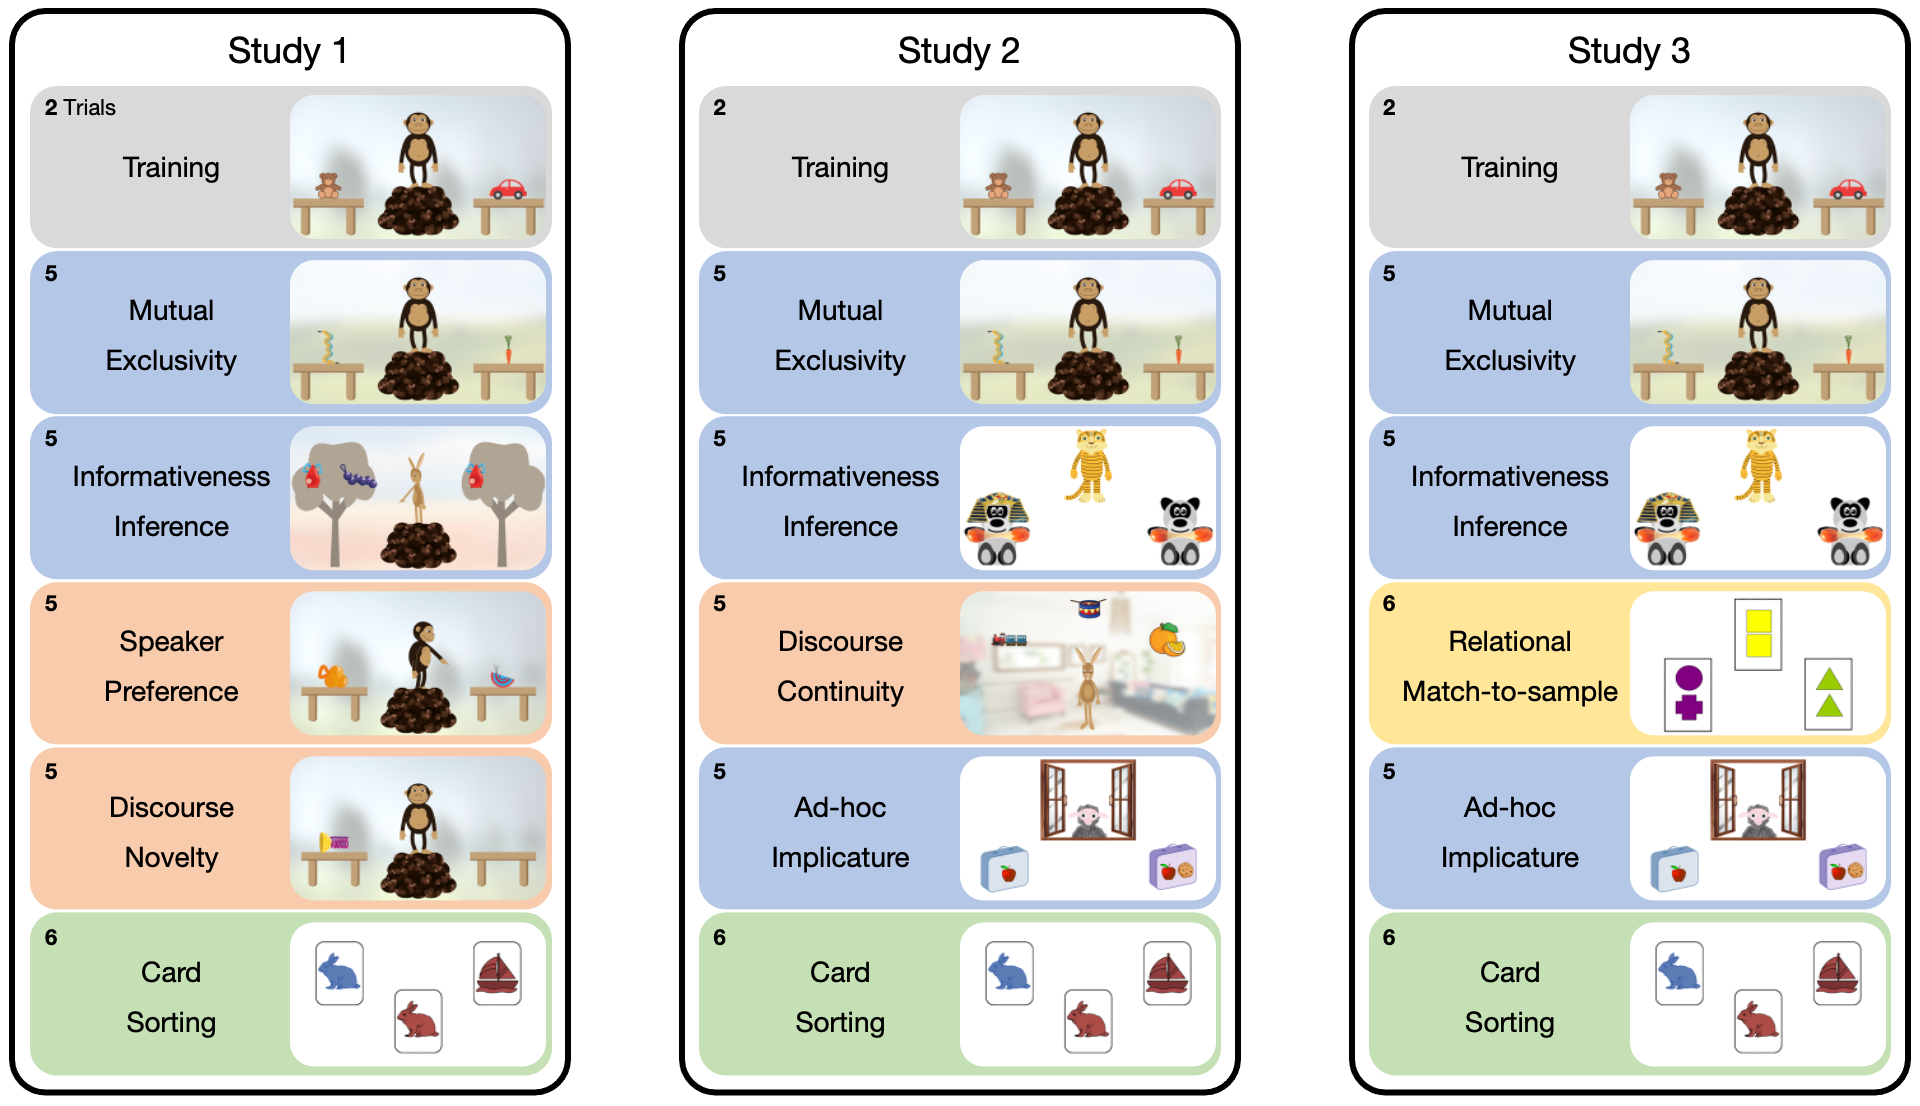
\includegraphics[width=1\linewidth]{./figures/figure1} 

}

\caption{Overview of the tasks used in Study 1 to 3. Pictures show screenshots from each task. The vertical order corresponds to the order of presentation in each study. The colors group the tasks along the (Assumed) cognitive processes involved. Blue: utterance-based inferences. Red common ground/discourse-based inferences. Green: Executive functions. Yellow: Analogical reasoning.}\label{fig:fig1}
\end{figure}

The study was presented as an interactive picture book on a tablet computer (Frank, Sugarman, Horowitz, Lewis, \& Yurovsky, 2016). The tasks were programmed in \texttt{HTML/JavaScript} and run in a web browser. Pre-recorded sound files were used to address the child (one native German speaker per animal). Children responded by touching objects on the screen. Children were tested in a quiet room in their daycare or in a separate room in a child laboratory. An experimenter guided the child through the study, selecting the different tasks and advancing within each task. In the beginning of the study, children completed a touch training to familiarize themselves with selecting objects. After a short introduction to the different animal characters, children completed the following six tasks. Figure \ref{fig:fig1} shows screenshots for each task and the order in which they were presented.

\hypertarget{training}{%
\subsubsection{Training}\label{training}}

An animal was standing on a pile between two tables. On each table, a familiar object was located. The animal asked the child to give them one of the objects (e.g., ``Can you give me the car''). the objects were chosen so that children of the youngest age group would easily understand them (car and ball). This procedure familiarized the child with the general logic of the animals making requests and the child touching objects. There were two training trials.

\hypertarget{mutual-exclusivity}{%
\subsubsection{Mutual exclusivity}\label{mutual-exclusivity}}

This task was directly taken from Bohn, Tessler, Merrick, and Frank (2021). The task layout and the procedure was the same as in the training. In each trial, one object was a novel object (drawn for the purpose of this study) while the other one was likely to be familiar to children. Both object types changed from trial to trial. Following Bohn et al. (2021), the familiar objects varied in terms of the likelihood that they would be familiar to children in the age range (carrot, duck, eggplant, garlic, horseshoe). For example, we assumed that most 3-year-olds would recognize a carrot, whereas fewer children would recognize a horseshoe. The animal always used a novel non-word (e.g., gepsa) in their request. We reasoned that children would identify the novel object as the referent of the novel word because they assumed the animal would have used the familiar word if they wanted to request the familiar object. Children's response was thus coded as correct if they selected the novel object. There were five trials, with the side on which the novel object appeared pseudo-randomized.

\hypertarget{informativeness-inference}{%
\subsubsection{Informativeness inference}\label{informativeness-inference}}

The task was directly taken from Bohn, Tessler, Merrick, and Frank (2022). Th animal was standing between two trees with objects hanging in them. In one tree, there were two objects (type A and B) and in the other tree there was only one (type B). The animal turned to the tree with the two objects and labelled one of the objects. It was unclear from the animal's utterance, which of the two objects they were referring to. We assumed that children would map the novel word onto the object of type A because they expected the animal to turn to the tree with only the object of type B if their intention was to provide a label for an object of type B. Next, the trees were replaced by new ones, one of which carried an object of type A and the other of type B. The animal then said that one of the trees had the same object as they labelled previously (using the same label) and asked the child to touch the tree. We coded as correct if the child selected the tree with the object of type A. The first two trials were training trials, in which there was only one object in each tree. There were five test trials. The location of the tree with the two objects in the beginning of each trial was pseudo-randomized and so was the location of the objects when the new trees appeared.

\hypertarget{speaker-preference}{%
\subsubsection{Speaker preference}\label{speaker-preference}}

This task was also taken from Bohn et al. (2022). The animal was standing between the two tables, each of which had a novel object (drawn for the purpose of the study) on it. The animal turned to one table, pointed at the object and said that they very much liked this object (using a pronoun instead of a label). Next, the animal turned to the other table and said that they really did not like the object (again, using a pronoun and no label). Then the animal turned towards the participant and used a novel label to request an object in an excited tone. We assumed that children would track the animal's preference and identify the previously liked object as the referent. Thus, we coded as correct if the child selected the object the animal expressed preference for. There were five test trials. The location of the preferred object as well as whether the animal first expressed liking or disliking was pseudo-randomized across trials

\hypertarget{discourse-novelty}{%
\subsubsection{Discourse novelty}\label{discourse-novelty}}

This task was taken from Bohn et al. (2021). Once again, the animal was standing between the two tables. One table was empty whereas there was a novel object on the other table. The animal turned towards the empty table and commented on its emptiness. Next, the animal turned to the other table and commented (in a neutral tone) on the presence of the object (not using a label). The animal then briefly disappeared. In the absence of the animal a second novel object appeared on the previously empty table. Then the animal returned and, facing the participant, asked for an object in an excited tone. We assumed that children would track which object was new to the ongoing interaction and identify the object that was new in context as the referent. We coded as correct when children selected the object that appeared later. There were five test trials. The location of the empty table and whether the animal first commented on the presence or absence of an object was pseudo-randomized across trials

\hypertarget{card-sorting}{%
\subsubsection{Card sorting}\label{card-sorting}}

This task was modeled after Zelazo (2006). The child saw to cards, a blue rabbit on the left and a red boat on the right. The experimenter introduced the child to the color game they would be playing next. In this game, all blue cards (irrespective of object depicted) would go to the left card and all red cards to the right. Next, a third card appeared in the middle of the screen (red rabbit or blue boat) and the experimenter demonstrated the color sorting by moving the card to the one with the same color. After a second demonstration trial, the child started to do the color sorting by themselves. After six trials, the experimenter said that they were now going to play a different game, the shape game, according to which all rabbits would go to the card with the rabbit (left) and all boats to the card with the boat (right). The experimenter repeated these instructions once and without any demonstration the child continued with the sorting according to the new rule. There were six test trials. The shape on the card was pseudo-randomized across trials. We only coded the trials after the rule change and coded as correct when the child sorted according to shape.

Each child received exactly the same version of each task and completed the tasks in the same order, with the same order on the two days. This ensured comparability of performance across children.

\hypertarget{analysis}{%
\subsection{Analysis}\label{analysis}}

We analysed the data in three steps. First we investigated developmental effects in each task, then we assessed re-test reliability and finally, we looked at relations between the tasks.

All analysis were run in \texttt{R} (R Core Team, 2018) version 4.1.2. Regression models were fit as Bayesian generalized linear mixed models (GLMM) using the function \texttt{brm} from the package \texttt{brms} (Bürkner, 2017). We used default priors for all analysis.

To estimate developmental effects in each task, we fit a GLMM predicting correct responses (0/1) by age (centered at the mean) and trial number (also centered). The model included random intercepts for each participant and random slopes for trial within participants (model notation in \texttt{R}: \texttt{correct\ \textasciitilde{}\ age\ +\ trial\ +\ (trial\textbar{}id)} ). For each task, we inspected and visualized the posterior distribution (mean and 95\% Credible Interval (CrI)) for the age estimate.

We assessed re-test reliability in two ways. First, for each task we computed the proportion of correct trials for each individual in the two test sessions and then used Pearson correlations to quantify re-test reliability. Second, we used a GLMM based approach suggested by Rouder and Haaf (2019). Here, a GLMM was fitted to the trial-by-trial data for each task with a fixed effect of age, a random intercept for each participant and a random slope for test day (\texttt{correct\ \textasciitilde{}\ age\ +\ (0+test\_day\textbar{}id)})\footnote{The notation \texttt{0+test\_day} yields a separate intercept estimate for each test day and subject instead of an intercept estimate for day 1 and a slope for the difference between day 1 and day 2. As a consequence, the model estimates the correlation between the two test days instead of a correlation between an intercept and the slope for test day.}. The model yields a participant specific estimate for each test day and also estimates the correlation between the two. This correlation can be interpreted as the re-test reliability. This approach has several advantages. First, it uses the trial-by-trial data and avoids information loss that comes with data aggregation. Second, it uses hierarchical shrinkage to obtain better participant specific estimates. Finally, it allows us to get an age-independent estimate for reliability. One worry when assessing re-test reliability in developmental studies is that re-test correlations can be high because of domain general cognitive gains and not because of task-specific individual differences. By including age as a fixed effect in the model, the estimates for each participant are independent of age and so is the correlation between estimates for the two test days -- the re-test reliability.

Finally, we used that aggregated data from both test days for each participant and task to compute Pearson correlations between the different tasks. Given the small sample size in Study 1, this part of the analysis is mostly exploratory.

\hypertarget{results}{%
\subsection{Results}\label{results}}



\begin{figure}

{\centering 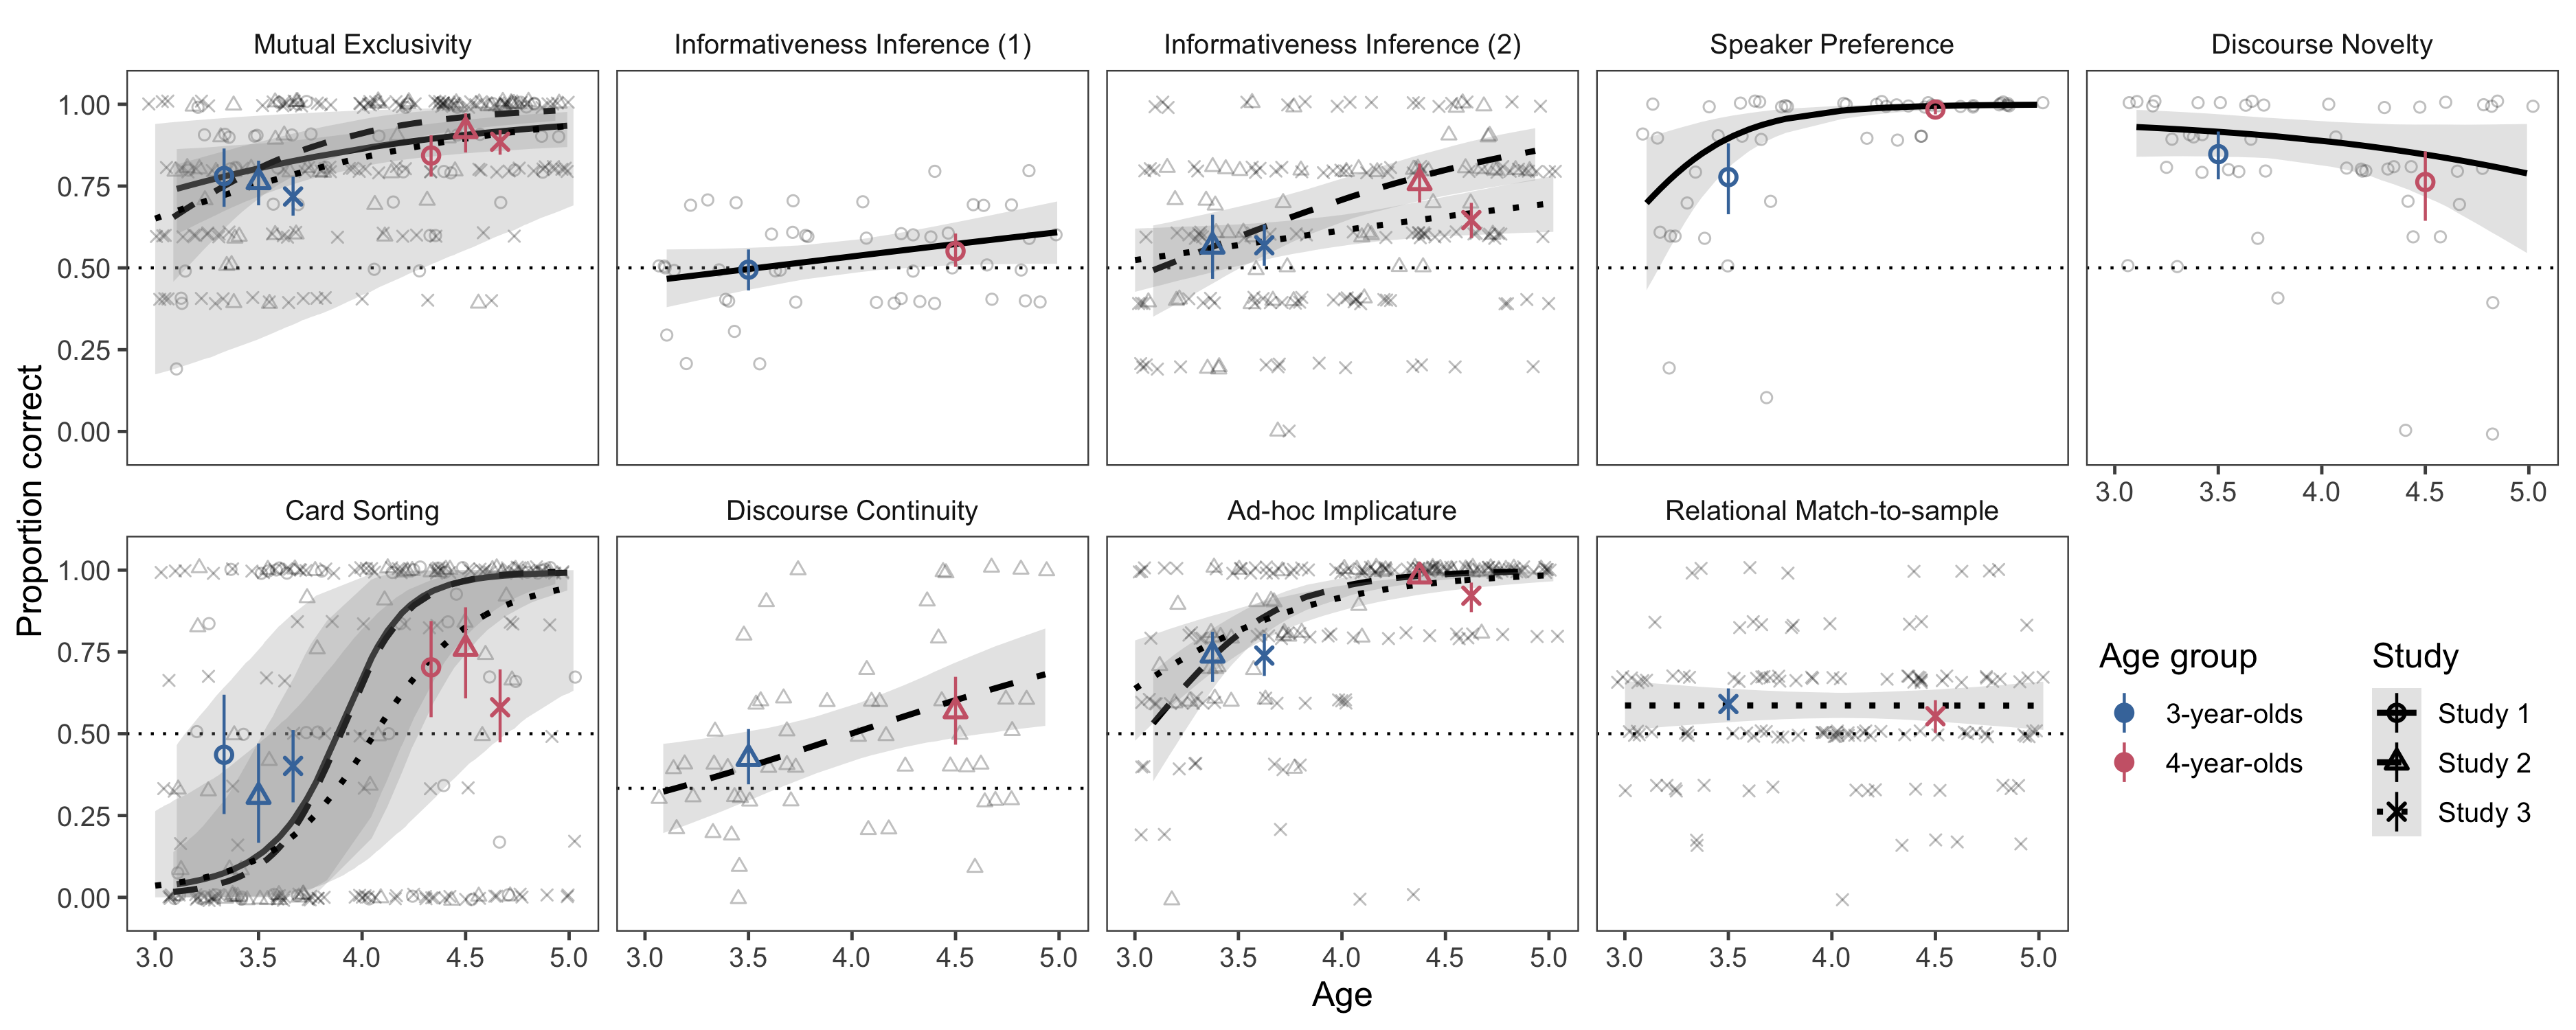
\includegraphics[width=1\linewidth]{./figures/figure2} 

}

\caption{Results by task for studies 1 to 3. Each panel shows the results for one task. Regression lines show the predicted developmental trajectories (with 95\% CrI) based on by-task GLMMs, with the line type indicating the study. Colored points show age group means (with 95\% CI based on non-parametric bootstrap) with the different shapes corresponding to the different studies. Light shapes show the mean performance for each subject by study. Dotted line shows level of performance expected by chance.}\label{fig:fig2}
\end{figure}

We found developmental effects in most of the tasks. Figure \ref{fig:fig2} shows the data and visualizes the developmental trajectories based on the model. Figure \ref{fig:fig3} shows the model estimates for age. In the mutual exclusivity task, performance was reliably above chance level and increased with age. For informative inference, the pattern was quite different: Performance was at chance level with only minor developmental gains. In the speaker preference task, performance was again clearly above chance with developmental gains resulting in a ceiling effect for older children. In the discourse novelty task, performance was also above chance with no clear developmental effects. The card sorting task showed the strongest developmental effects with younger children performing largely below chance and older children performing above chance.

Re-test reliability was high for most tasks (see Figure \ref{fig:fig2}). Raw correlations between the two test sessions was above .7 for mutual exclusivity, speaker preference and discourse novelty. With .62 it was slightly lower for card sorting. The model based -- age independent -- reliability estimates yielded similar results suggesting that the tasks did capture task specific individual differences. A notable exception was the informativeness inference task, which was not reliable according to any of the methods of computing re-test correlations. We suspect the overall low variation in performance to be responsible for this.

Most correlations between the tasks were low and ranged between \emph{r} = -0.2 and 0.2 (see Figure \ref{fig:fig2}). A notable exception was the correlation between mutual exclusivity and card sorting with \emph{r} = 0.31 (95\% CI{[}0.03 - 0.55{]}).



\begin{figure}

{\centering 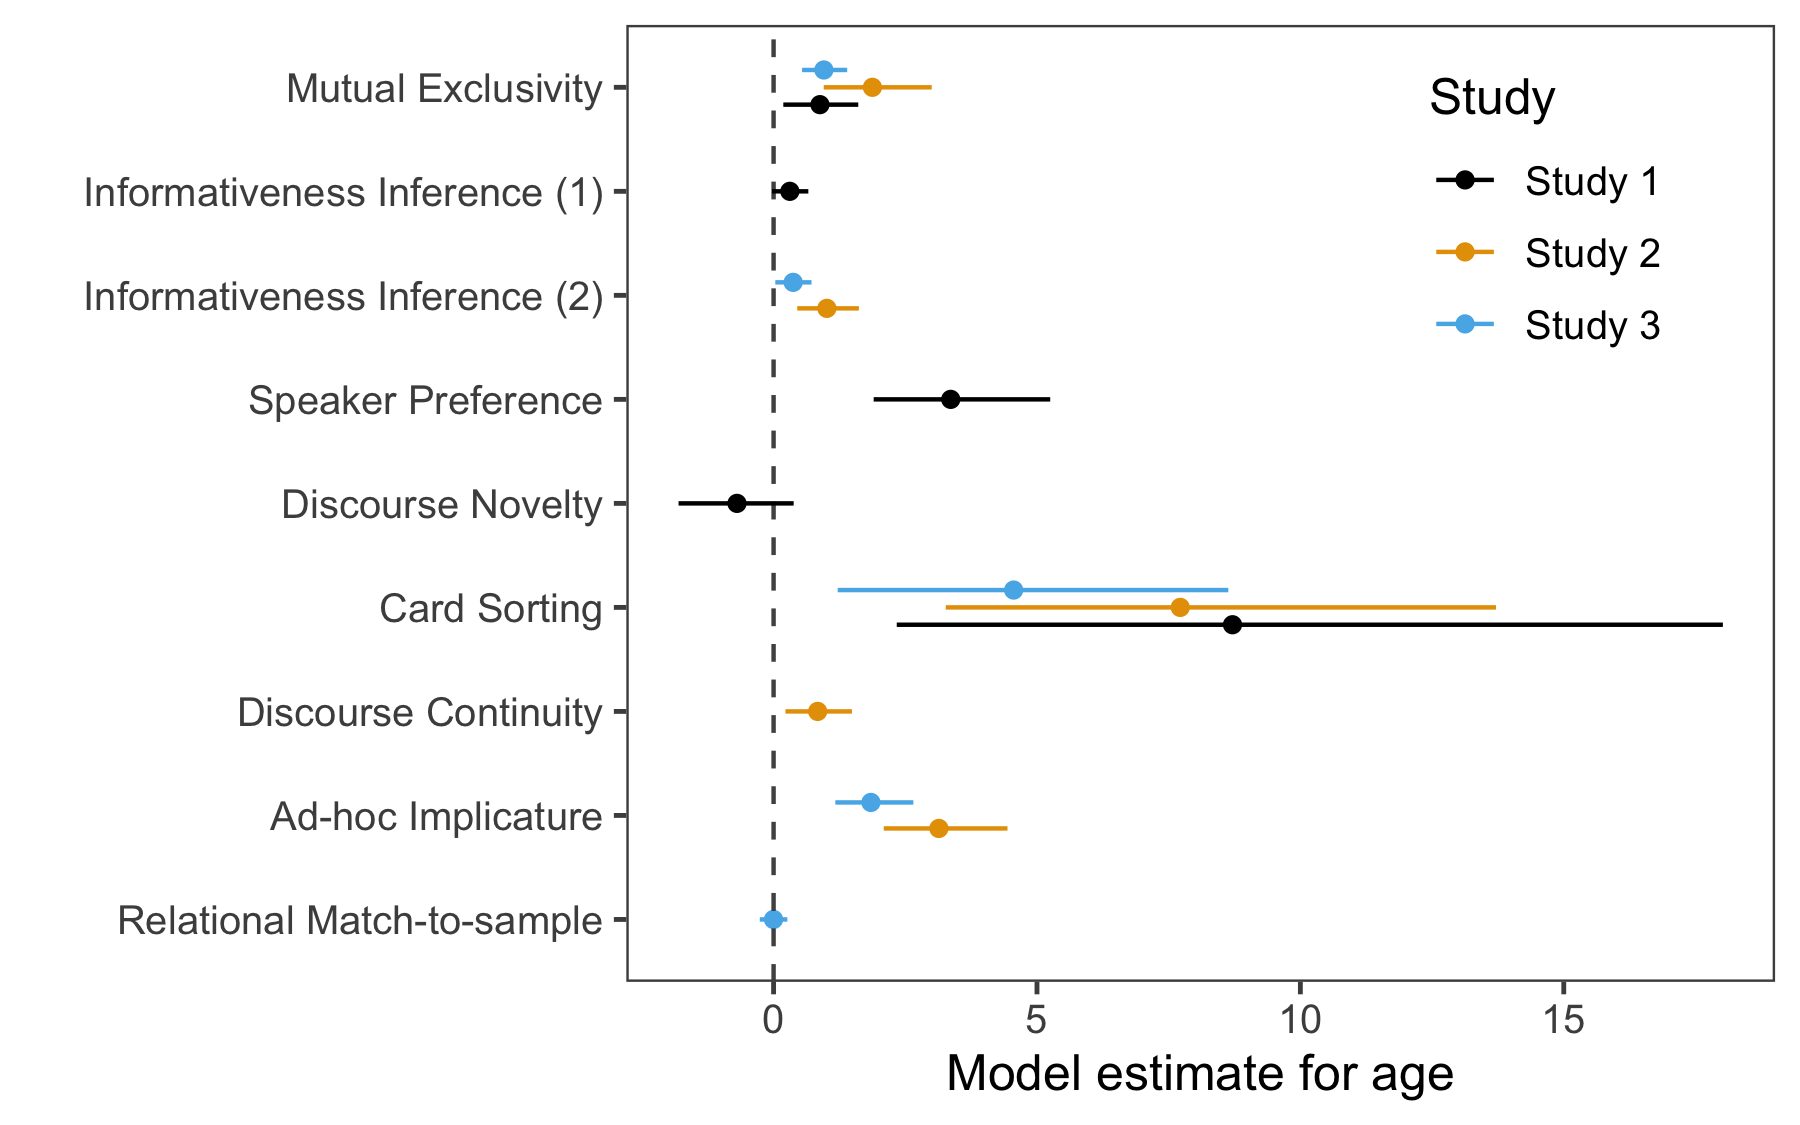
\includegraphics[width=0.6\linewidth]{./figures/figure3} 

}

\caption{Model estimates (with 95\% CrI) for age based on GLMMs for each task and study.}\label{fig:fig3}
\end{figure}



\begin{figure}

{\centering 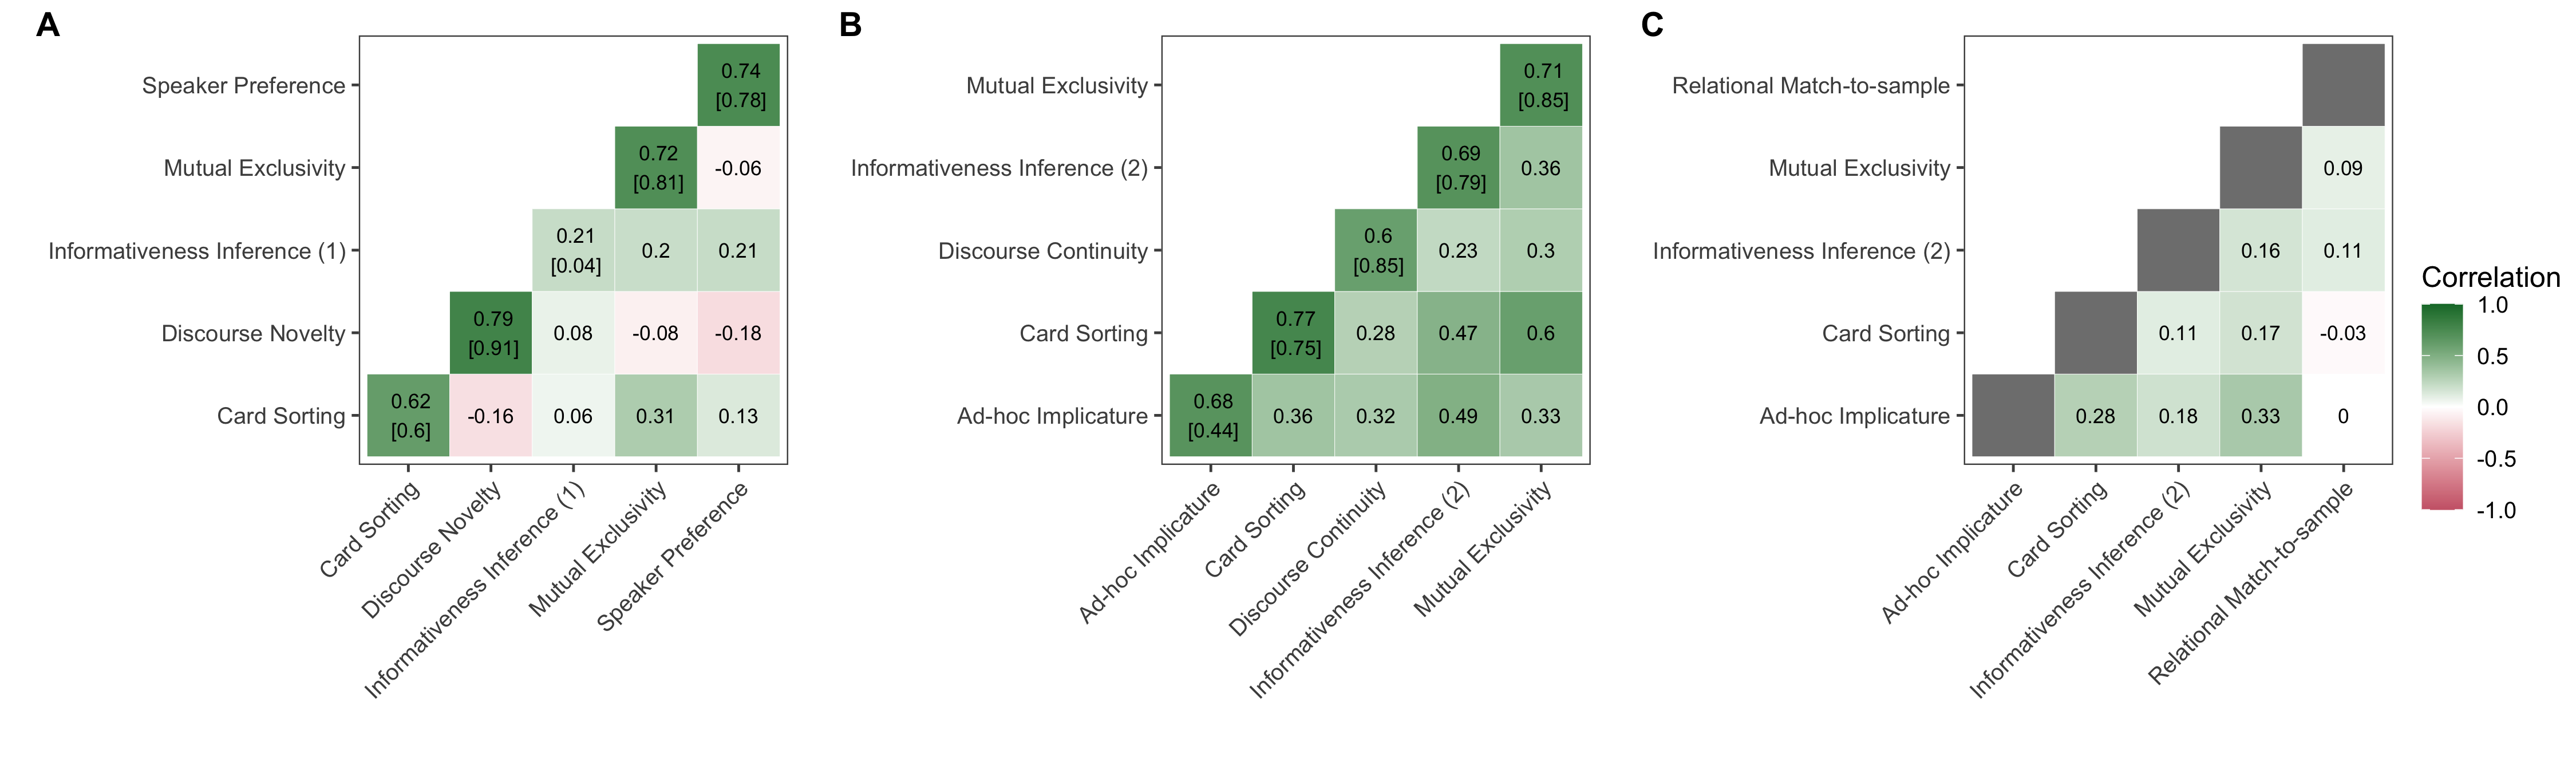
\includegraphics[width=1\linewidth]{./figures/figure4} 

}

\caption{Re-test and task correlations for Study 1 (A), 2 (B) and 3 (C). The diagonal in A and B shows the re-test reliability based on aggregated raw test scores (top row) and based on a GLMM that accounted for participant age (see main text for details).}\label{fig:fig4}
\end{figure}

\hypertarget{discussion}{%
\subsection{Discussion}\label{discussion}}

Study 1 showed that the different tasks were age appropriate and reliable. A notable exception was the informativeness inference task which generated to systematic variation in the age range we studied here. Correlations between the tasks were generally low, with the notable exception of the relation between mutual exclusivity and card sorting. Given the small sample size, we want to avoid overly strong claims, however, it was interesting to see that the relation between the two tasks tapping into common ground based inferences (speaker preference and discourse novelty) were -- if anything -- negatively correlated.

\hypertarget{study-2}{%
\section{Study 2}\label{study-2}}

Based on these results od Study 1, we compiled a new set of tasks for Study 2. We retained the mutual exclusivity and card sorting tasks because of the interesting relation between the two found in Study 2. We simplified the informativeness inference task to be more age appropriate with the hope to induce more variation in performance. We removed the speaker preference and discourse novelty tasks -- despite their excellent re-test reliability -- because they seemed to be unrelated to one another and also unrelated to the other tasks. The new tasks focused on ad-hoc implicature and discourse continuity. As noted in the introduction, we had theoretical reasons to expected the ad-hoc implicature task to be related to the mutual exclusivity and informativeness inference tasks. We had no such strong predictions for the discourse continuity task.

Methods and sample size were pre-registered at \url{https://osf.io/hp9f7}. Data, analysis scripts and experiment code can be found in the associated online repository.

\hypertarget{participants-1}{%
\subsection{Participants}\label{participants-1}}

Participants for Study 2 were recruited from the same general population. We collected data from 54 children (\(m_{age}\) = 3.97, range\(_{age}\): 3.09 - 4.93, 24 girls) of which 40 were tested twice. The two test sessions were again two days apart; the longest time difference was 14 days. Data was collected between March and October 2020.

\hypertarget{material-and-methods-1}{%
\subsection{Material and Methods}\label{material-and-methods-1}}

The general setup and mode of presentation was the same as in Study 1. We added two new tasks and modified the informativeness inferences task, which we will describe in detail below. The mutual exclusivity and card sorting tasks were the same as in Study 1.

\hypertarget{informativeness-inference-1}{%
\subsubsection{Informativeness inference}\label{informativeness-inference-1}}

The general structure of the task was the same as in Study 1, however, we replaced the stimuli by the ones used by Frank and Goodman (2014). We suspected that children did not treat the novel objects hanging in the tree as properties of the tree but the tree as a ``container'' for the novel objects. The alleged inference, however, relies on seeing the objects as properties of the referent. With the new stimuli, we emphasized that the novel objects were mere properties of the referent by making the referent more salient and more different across trials. The animal was located between two identical objects, which had different properties (see Figure \ref{fig:fig1}). For example, the child saw two bears, one with a Pharaoh-style crown and a match in its hand, the other only with the match. The animal then turned to the object with the two properties and described it by referring to one of the properties (e.g., a bear with a {[}non-word{]}). Next, the objects disappeared, and the same objects re-appeared but this time, each of them had only one property (e.g., one bear with a crown, the other with the match). The animal then asked which of these objects had the aforementioned property (e.g., which bear has a {[}non-word{]}). We coded as correct if the child selected the object with the property that was unique to the object during labeling. The first two trials were training trials, in which each object only had one property. There were five test trials. The location of the object with the two properties in the beginning of each trial was pseudo-randomized and so was the location of the properties when the new objects appeared.

\hypertarget{discourse-continuity}{%
\subsubsection{Discourse continuity}\label{discourse-continuity}}

This task was directly taken from Bohn et al. (2021). Children were told that they were going to visit the animals at their place. The animal greeted the child and told them that they would show them their things. During exposure trials, the child saw three objects from three different categories (e.g., train (vehicle), drum (instrument), orange (fruit); see Figure \ref{fig:fig1}). The animal named of the objects and asked the child to touch it. On the next exposure trial, the child saw three new objects but from the same categories (e.g., bus (vehicle), flute (instrument), apple (fruit)). The animal asked the child to touch the object from the same category as previously (only naming the object, not the category). There were 5 such exposure trials. On the following test trial, the animal used a pronoun to refer to one of the objects (i.e., can you touch \emph{it}). We assumed that children would use the exposure trials to infer that the animal was talking about a certain category and would use this knowledge to identify the referent of the pronoun.Children received five test trials, each with a different category as the target. The position of the objects in exposure trials as well as test trials was pseudo-randomized.

\hypertarget{ad-hoc-implicature}{%
\subsubsection{Ad-hoc implicature}\label{ad-hoc-implicature}}

This task used the general procedure and stimuli developed in Yoon and Frank (2019). The animal was located in a window, looking out over two objects (see Figure \ref{fig:fig1}). Both objects were of the same kind, but had different properties. As properties we chose objects that were well known to children of that age range. One object had one property (A) and while the other had two (A and B). For example, objects were lunchboxes, one with an orange and the other with an orange and an apple. The animal then asked the child to hand them their object which was the one with the property that both objects shared (A). We assumed that children would pick the object with only property A because they expected the animal to name property B if they had wanted to refer to the object with both properties. There were five test trials, preceded by two training trials in which the objects did not share a common property. The positioning of the objects (left and right) was pseudo-randomized

\hypertarget{analysis-1}{%
\subsection{Analysis}\label{analysis-1}}

We used the same methods to analyse the data as in Study 1.

\hypertarget{results-1}{%
\subsection{Results}\label{results-1}}

We found substantial developmental gains in all five tasks (Figure \ref{fig:fig2} and \ref{fig:fig3}). For mutual exclusivity and ad-hoc implicature performance was above chance across the entire age range. For the informativeness inference and discourse continuity tasks, performance was close to chance for younger children and reliably above it for older children. Like in Study 1, we found the strongest developmental effect for card sorting, with performance below chance for 3-year-olds and above chance for 4-year-olds.

Re-test reliability based on aggregated data was good for all tasks with most estimates around 0.7. The model-based reliability estimates were similar, with lower values for ad-hoc implicature and higher ones for discourse continuity. Notably, the informativeness inference task showed a much-improved re-test reliability compared to Study 1.

Correlations between tasks were generally higher compared to Study 1. In fact, confidence intervals for correlation coefficients were not overlapping with 0 except for the correlation between the discourse continuity and informativeness inference tasks (Figure \ref{fig:fig4}. Once again, we found the strongest relation between card sorting and mutual exclusivity (\emph{r} = 0.60, 95\% CI{[}0.40 - 0.75{]}). Other notable relations were those between card sorting and informativeness inference (\emph{r} = 0.47, 95\% CI{[}0.23 - 0.65{]}) as well as between ad-hoc implicature and informativeness inference (\emph{r} = 0.49, 95\% CI{[}0.25 - 0.67{]}).

\hypertarget{discussion-1}{%
\subsection{Discussion}\label{discussion-1}}

In Study 2 we found good results from a measurement perspective: all tasks had acceptable re-test reliability. This included the informativeness inference task which had deficits in that respect in Study 1. Higher average performance and increased variability suggest that our changes to the stimuli did make the task easier for children.

Like in Study 1, we found a relatively strong correlation between the mutual exclusivity and card sorting tasks. This corroborates the idea that these tasks share common processes. We also found substantial relations between the three utterance-based inference tasks (mutual exclusivity, ad-hoc implicature, informativeness inference). Furthermore, the correlations between tasks were lower when discourse continuity was involved -- though the numerical difference was minimal.

\hypertarget{study-3}{%
\section{Study 3}\label{study-3}}

In Study 3, we focused explicitly on the relations between the different tasks. In particular, we explored the idea that the three utterance-based inference tasks share common cognitive processes. Once again, we also included the card sorting task and added a new task of analogical reasoning for which we did not expect strong relations with the other tasks. To be able to test these predictions, we collected data from a comparatively larger sample of children.

The reliability estimates from Study 1 and 2 helped us plan the sample size for Study 3. The focal tasks had a re-test reliability around 0.7. Because the highest plausible correlation between two tasks is the product of their reliabilities (higher correlations would mean that the task is more strongly related to a different task than to itself), the highest we could expect were correlations between two tasks around 0.7 * 0.7 = 0.49. We planned our sample so that we could detect correlations between two tasks of 0.3 with 95\% power\footnote{The first author drafted a pre-registration and shared it with the last author but forgot to register it at OSF. Thus, the study was not officially pre-registered.}. Data, analysis scripts and experiment code can be found in the associated online repository.

\hypertarget{participants-2}{%
\subsection{Participants}\label{participants-2}}

For Study 3, we collected data from 126 children (\(m_{age}\) = 4.00, range\(_{age}\): 3.00 - 5.02, 74 girls) from the same general population. Data was collected between June and November 2021. Children were tested only once.

\hypertarget{materials-and-methods}{%
\subsection{Materials and Methods}\label{materials-and-methods}}

From Study 2, we used the the mutual exclusivity, ad-hoc implicature, informativeness inference and card sorting tasks. We added the relational match-to-sample task, which we now describe in more detail.

\hypertarget{relational-match-to-sample}{%
\subsubsection{Relational match-to-sample}\label{relational-match-to-sample}}

The task was modeled after and used the original stimuli from Christie and Gentner (2014). The child saw three cards, one on top (the sample) and two at the bottom (the potential matches; see Figure \ref{fig:fig1}). The experimenter guided the child through the study and read out the instructions. The child was instructed to match the sample card to one of the lower ones based on similarity, that is, they were instructed to pick the card that was ``like'' the sample. All cards had two geometrical shapes of the same color on them. The sample card showed to identical shapes and so did one of the potential matches. The other card showed two different shapes. We assumed that children would match the sample to the match that showed the same relation between shapes (sameness). Children received six test trial, preceded by two training trials in which one of the potential matches was identical to the sample. The position of the same-match was pseudo randomized.

\hypertarget{analysis-2}{%
\subsection{Analysis}\label{analysis-2}}

Study 3 had only one test session. Therefore, we did not investigate re-test reliability. We estimated age effects and raw correlations between tasks in the same way as in Studies 1 and 2. We used two additional methods to investigate the structure of individual differences between tasks.

First, we used Confirmatory Factor Analysis (CFA). Models were fit in a Bayesian framework using the \texttt{R} package \texttt{blavaan} (Merkle \& Rosseel, 2018) using default priors. As outlined above, our focal model assumed that mutual exclusivity, ad-hoc implicature and informativeness inference load on a common pragmatics factor. The card sorting and relational match-to-sample tasks were included as separate factors. We used Posterior Predictive P-Values (PPP) to evaluate model fit (Lee \& Song, 2012). A good model fit is indicated by a PPP close to 0.5 and should not be smaller than 0.1 (Cain \& Zhang, 2019). We also fit two alternative models: one including only a single factor on which all tasks loaded and a second with a separate factor for each task. We compared models using WAIC (widely applicable information criterion) scores and weights (McElreath, 2018). WAIC is an indicator of out-of-sample predictive accuracy with lower values indicating better fit. WAIC weights transform WAIC values to give the probability that a particular model (out of the models considered) provides the best out-of-sample predictions. Within the focal model, we inspected the posterior estimates (with 95\%CrI) for the factor loadings and the variance in the task explained by the factor for the three pragmatics tasks. In addition, we evaluated the correlations between the pragmatics factor and the other two tasks.

Second, we used computational cognitive models from the Rational Speech Act (RSA) framework to relate the three pragmatics tasks to one another (Frank \& Goodman, 2012; Goodman \& Frank, 2016). In contrast to the CFA model above, the RSA models are models of the tasks, and not of the data. That is, they include a schematic representation of the experimental tasks and provide a computational account of how participants make inferences in this context. RSA models see pragmatic inferences as a form of Bayesian social reasoning where the listener tries to infer the speaker' meaning (here: the intended referent) by assuming that the speaker is helpful and informative. Being helpful and informative means that the speaker chooses a message based on the probability that it would help the listener would recover the speaker's intended meaning. Thus, RSA models have a recursive structure in which the the listener reasons about a speaker who is reasoning about the listener. To avoid an infinite regress, the speaker is assumed to reason about a literal listener, who interprets words according to their literal semantics.

The studies from which we took the mutual exclusivity and informativeness inference tasks also formalized these tasks in an RSA-style model (Bohn et al., 2021, 2022). We refer to this earlier work for more details and a mathematical description of the models. For the present study, we formalized the ad-hoc implicature task within the same RSA framework. The three models share the same contrastive inference process according to which the listener compares the speaker's utterance to alternative, possible ones. The speaker then expects the listener to be informative (with degree \(\alpha\)), that is, choose the utterance that best communicates the intended message. In the mutual exclusivity task, the alternative utterance would be to use a familiar word. In the case of the informative inference task, the alternative was point to the object with only one property. For the ad-hoc implicature task it was to single out the property that was shared by both objects. In all cases, these alternative utterances would be better suited to communicate about the respective other referent.

As noted above, all models shared one common parameter: the speaker informativeness parameter \(\alpha\). This commonality offers a way of relating performance in the three tasks to one another by constraining the three models to use the same value for \(\alpha\). We then used Bayesian inference to estimate the posterior distribution for \(\alpha\) that best explained performance in the three tasks. To adapt this framework to the study of individual differences, we allowed a separate parameter for each participant (\(\alpha_i\)). We estimated \(\alpha_i\) in a hierarchical model as a deviation from a hyper parameter: \(\alpha_i \sim \mathcal{N}(\alpha_j, \sigma^\alpha)\). Given the developmental nature of our data, we defined \(\alpha_j\) via a linear regression as a function of the child's age (\(age_i\)): \(\alpha_j = \beta^\alpha_0 + age_i \cdot \beta^\alpha_1\). Thus, the participant specific value for \(\alpha\) was not only constrained by the performance in the three tasks but also by the child's age.

To account for differences in difficulty between the tasks due to other factors, we added a scale parameter to the model that adjusted \(\alpha\) for each task in comparison to a reference task (ad-hoc implicature).

To validate this approach, we first applied this model to the data from Study 2 -- separate for each test session. This allowed us to compute the re-test reliability of \(\alpha\) and see if it captures individual differences equally well compared to the raw test scores. After finding excellent re-test reliability, we applied it to the data from Study 3 and correlated the results with the the card sorting and relational match-to sample tasks. For these correlational analysis, we converted the posterior distribution for each participant into a single value by taking the mode (and 95\% highest density interval -- HDI). The cognitive models were implemented in \texttt{WebPPL} (Goodman \& Stuhlmüller, 2014) and the corresponding code, including information on prior distributions, can be found in the associated online repository.

\hypertarget{results-2}{%
\subsection{Results}\label{results-2}}

The age effects in Study 3 largely replicate those of Study 2 for the four overlapping tasks (see Figure \ref{fig:fig2} and \ref{fig:fig3}. There were no substantial developmental gains in the newly added relational match-to-sample task and performance was close to chance for both age groups. Thus -- in the absence of information on re-test reliability -- it is unclear if the variation in performance reflects systematic individual differences in analogical reasoning or not.

Overall, the correlations between the tasks were lower compared to Study 2. This was to some extend expected given that there were only half the number of trials per task in Study 3 and, with that, less room for capturing individual differences. Nevertheless, the overall pattern rsembles that found in Study 2 (Figure \ref{fig:fig4}). We saw the strongest bi-variate relation between the mutual exclusivity and the ad-hoc implicature task (\emph{r} = 0.33, 95\% CI{[}0.16 - 0.48{]}) followed by ad-hoc implicature and card sorting (\emph{r} = 0.28, 95\% CI{[}0.11 - 0.44{]}). The relational match-to-sample task showed no substantial correlations with any of the other tasks.



\begin{figure}

{\centering 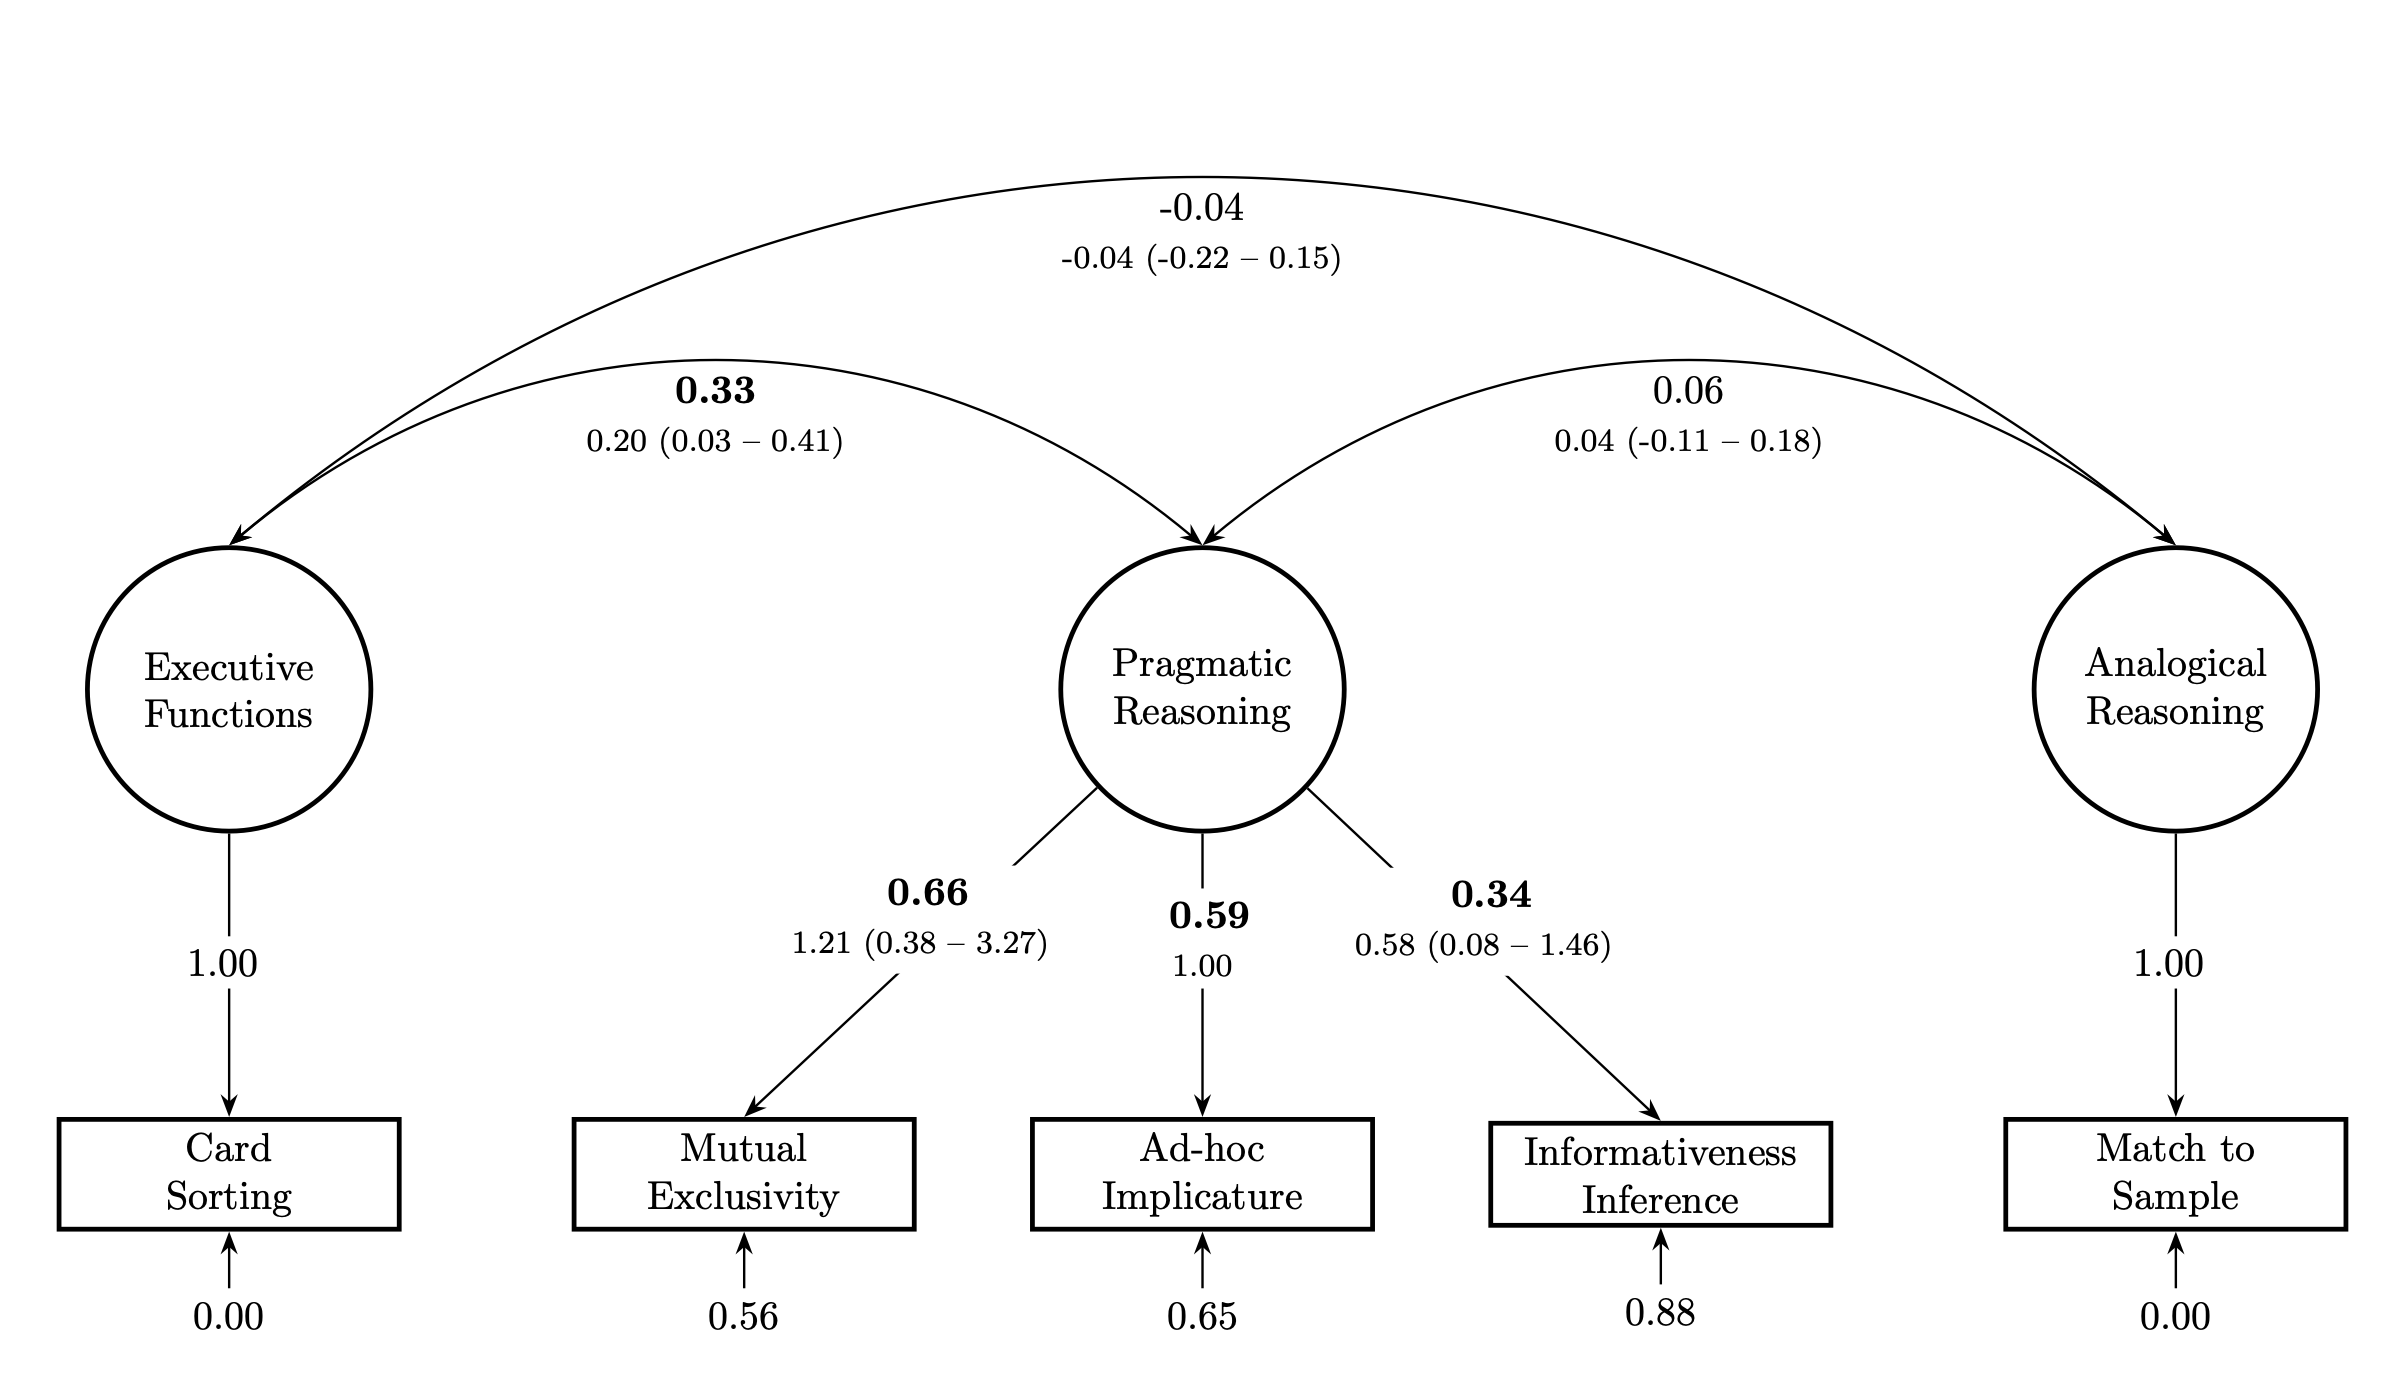
\includegraphics[width=1\linewidth]{./figures/figure5} 

}

\caption{Graphical overview of CFA model for Study 3. Arrows from latent variable (circles) to observed variable (rectangles) show factor loadings. Bottom arrows to observed variables give the residual variance not explained by the factor. Bent arrows between latent variables show correlations. Bottom rows show model estimates with 95\% CrI. Top rows show standardized estimates (bold if 95 \% CrI does not include 0).}\label{fig:fig5}
\end{figure}

Next, we turn to the results of the confirmatory factor analysis. Our focal model -- including a latent factor for pragmatic reasoning -- fit the data well (PPP = 0.50) and with a WAIC of 1,753.45 (se = 32.02, weight = 0.74) better compared to the two alternative models (individual factors model: PPP = 0.51, WAIC = 1,756.48, se = 32.51, weight = 0.16; one factor model: PPP = 0.36, WAIC = 1,758.10, se = 32.37, weight = 0.07). Figure \ref{fig:fig5} shows that factor loadings for the individual tasks as well as their residual variance. The latent pragmatic reasoning factor best explained the mutual exclusivity task, followed by the ad-hoc implicature and the informativeness inference task. The correlation between pragmatic reasoning and executive functions (indicated by the card sorting task) was estimated to be reliably different from zero (\emph{r} = 0.33; model estimate = 0.20, 95\% CrI {[}0.02 - 0.39{]}). There was no systematic relation between pragmatic reasoning and analogical reasoning (as indicated by the relational match-to-sample task): \emph{r} = 0.06; model estimate = 0.04, 95\% CrI {[}-0.11 - 0.18{]}. However, the latter result should be taken with a grain of salt given the unknown psychometric properties of the relational match-to-sample task.

Finally, we present the results of the cognitive modeling analysis. Using the data from Study 2, we could show that participant specific speaker informativeness parameters (\(\alpha\)) were highly reliable (Figure \ref{fig:fig6}B). The scale parameter suggested that the mutual exclusivity task was easier and the informativeness inference task was harder compared to the ad-hoc implicature task (Figure \ref{fig:fig6}C). When correlating \(\alpha\) with performance in the other two tasks, the cognitive modeling approach yielded similar conclusions compared to the confirmatory factor analysis (Figure \ref{fig:fig6}A): There was a substantial correlation with the card sorting (\emph{r} = 0.31, 95\% CI{[}0.15 - 0.47{]}) but not the relational match-to-sample task (\emph{r} = 0.03, 95\% CI{[}-0.15 - 0.20{]}). The same limitations apply to the latter result as for the confirmatory factor analysis.



\begin{figure}

{\centering 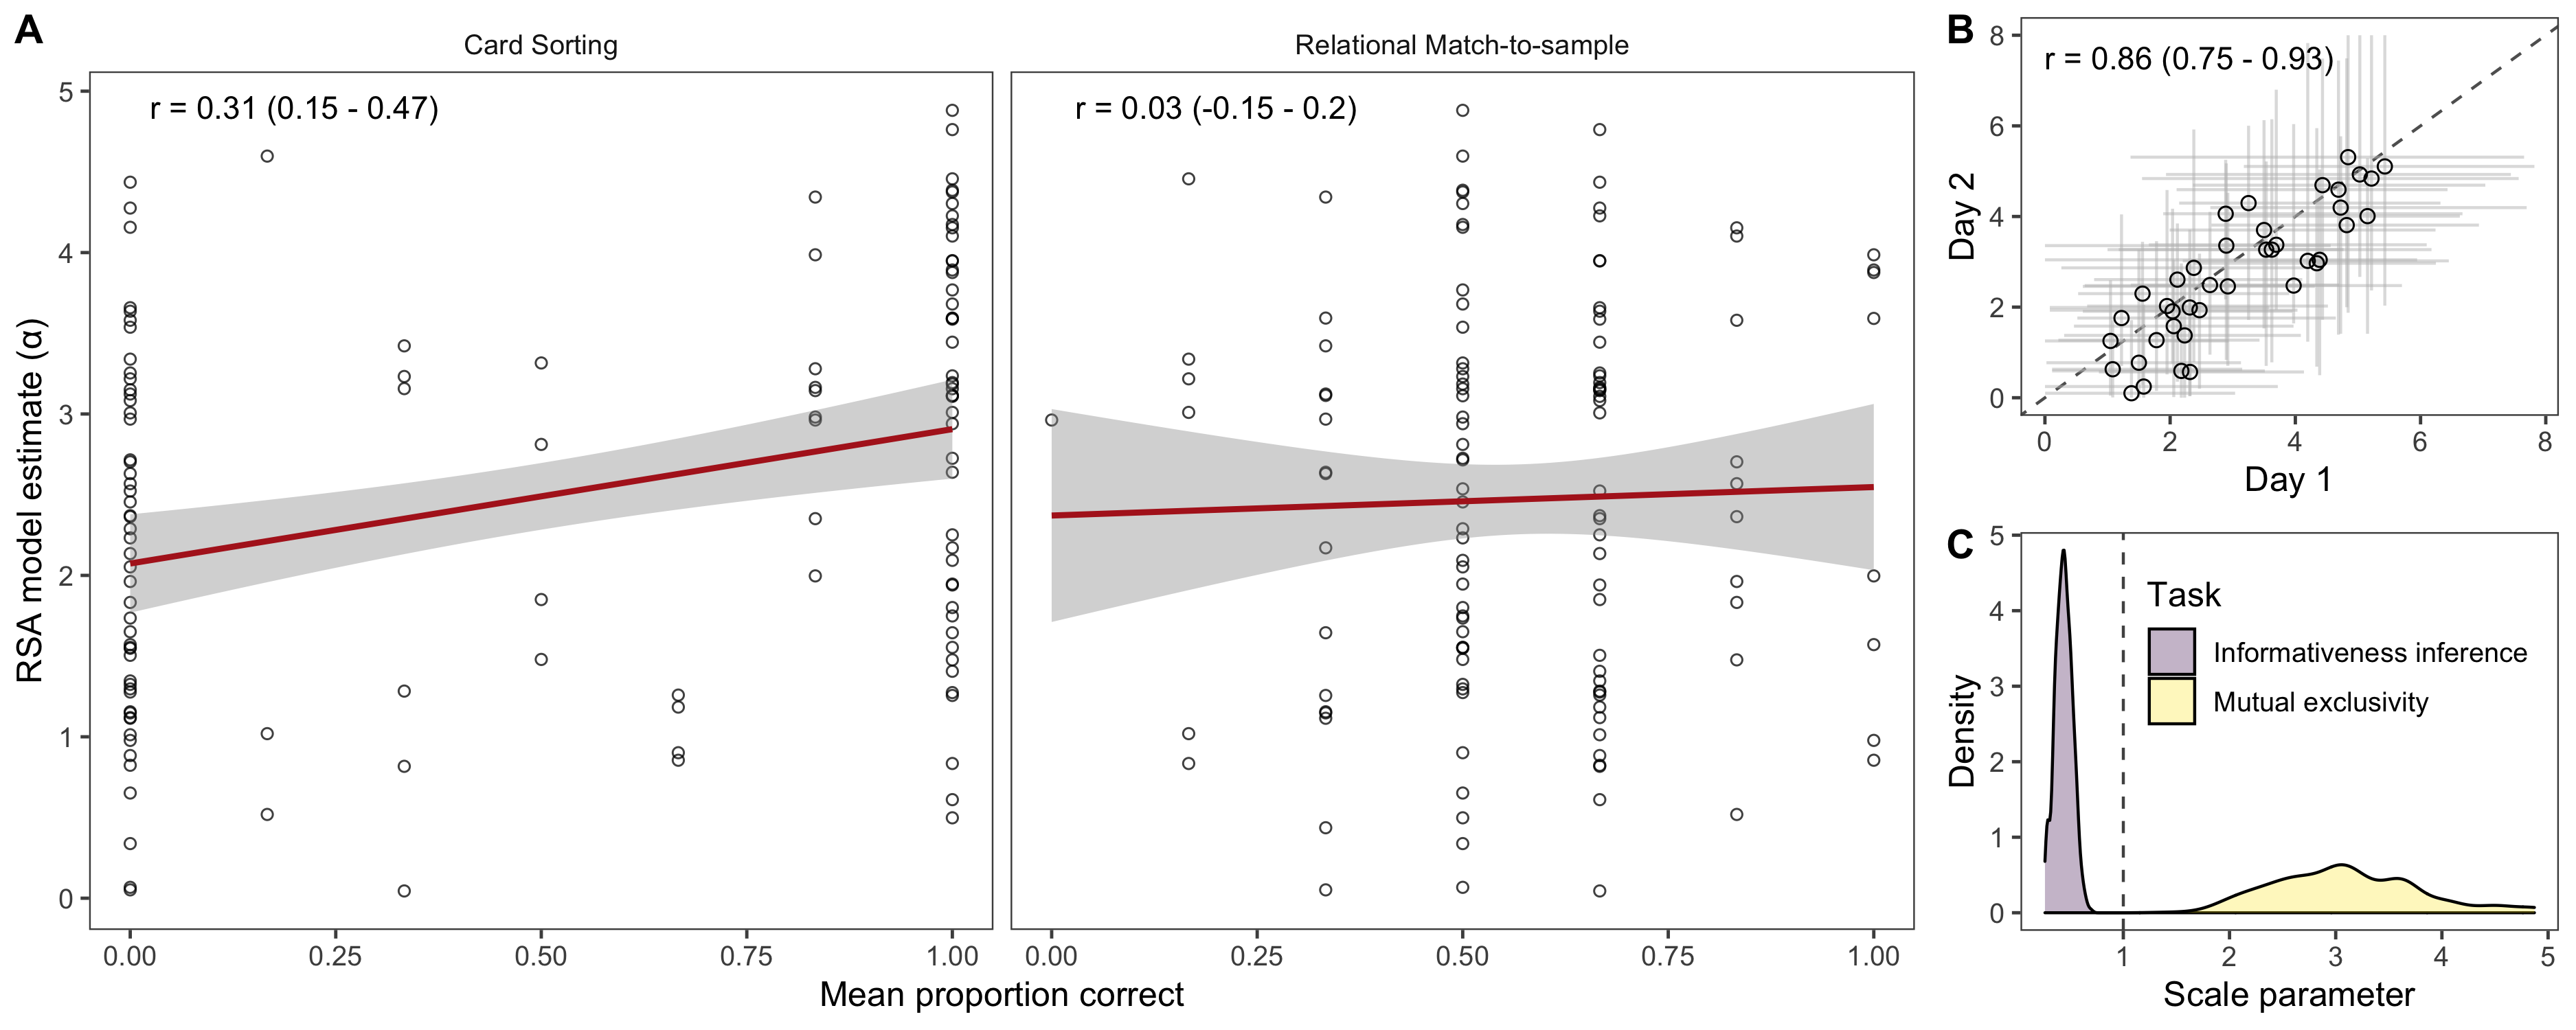
\includegraphics[width=1\linewidth]{./figures/figure6} 

}

\caption{Results of cognitive model analyses. A: Correlation between the speaker informativeness parameter \(\alpha\) and the paerformance in the card sorting and relational match to sample tasks. Regression line (with 95\% CI) is based on a linear model. B: Re-test reliability for \(\alpha\) based on the data from Study 2. C: Scale parameter for \(\alpha\) in relation to the ad-hoc implicature task. Values below 1 indicate a more difficult task, values above 1 an easier task. Correlation coefficients show Pearson correlation with 95\% CI.}\label{fig:fig6}
\end{figure}

\hypertarget{discussion-2}{%
\subsection{Discussion}\label{discussion-2}}

Using a diversity of different analytical tools, we found that performance in the three utterance-based pragmatic inference tasks was related in a way that points to shared cognitive processes. In the confirmatory factor analysis, we found that a model including a latent pragmatic reasoning factor fit the data well and better compared to alternative models. The latent factor explained substantial portions of the variance in each of the three tasks. The cognitive modelling approach provides an explicit theory of what the shared cognitive processes may look like: according to the model, the pragmatic inference in each task was driven by contrasting the utterance the speaker produced and alternative utterances. Individual differences were thought to arise from differential expectations about how informative the speaker is.

Both analytic strategies point to systematic relations between pragmatic reasoning and executive functions as indicated by the card sorting test. We found no such relations with analogical reasoning as indicated by the relational match-to-sample task. However, given the unknown psychometric properties of the latter task, this result should be interpreted with caution.

\hypertarget{general-discussion}{%
\section{General Discussion}\label{general-discussion}}

In this paper, we explored the development of pragmatic inferences in the preschool years. We identified six tasks covering a broad range of pragmatic phenomena. We found them to have good psychometric properties, in particular good to excellent re-test reliability. We then selected three utterance-based inference tasks for well-powered study of relations among different types of pragmatic abilities and between pragmatics and other cognitive processes. The results showed systematic relations between the tasks. We used a computational cognitive model of pragmatic reasoning to formalize the cognitive processes we believed the tasks to share. Finally, we found pragmatic abilities to be related to a task of executive functions.

One of the main contributions of this paper is that if presents six pragmatic inference tasks that are highly robust and reliable. Whenever we used a task in two studies (mutual exclusivity, informativeness inference, ad-hoc implicature), we found the developmental results to closely replicate. in Study 1 and 2, all tasks showed good re-test reliability -- even when corrected for age. A notable exception was the informativeness inference task in Study 1. However, after making some procedural changes, it turned out to be robust and reliable as well. Taken together, the tasks are highly suitable for individual differences research. The material is freely available via the online repository associated with the study.

We grouped the tasks into utterance-based and common ground/discourse based. This grouping broadly captured the kind of information that we assumed to be relevant to compute the inference. For Study 3, we focused on the three utterance-based tasks. The main reason was theoretical. We were able to build on earlier work and formalize the inferences involved in these tasks in a common computational framework. We specified the structural overlap between the tasks and identified a parameter in the model that we used to capture individual differences. The shared structural features involve a recursive social inference process according to which the listener expects the speaker to select the most informative of a set of possible utterances. The individual difference parameter captured how informative the listener expected the speaker to be\footnote{this interpretation follows from the conceptual role the parameter plays in the RSA framework. Technically, it acts as an amplifier of the basic inference}. Previous accounts, in particular of mutual exclusivity (reviewed in Lewis et al., 2020), would not have predicted such an overlap. The results of Study 3 (and also Study 2) supported our assumptions as we found systematic relations between the three tasks.

Our formal model also allows us to speculate about why we saw a systematic relation across the three studies between pragmatic inference and the card sorting task as a measure of executive functions. Before we do so, we want to emphasize that the model is first and foremost a computational description of the tasks an not a model of a psychological process (cf. Goodman \& Frank, 2016). For the following, we assume more psychological realism than perhaps warranted. The card sorting task asks the child to switch between rules half way. This requires inhibiting a previously dominant response and attending to different features of the cards. The pragmatic inference in the model involves contrasting the observed utterance with alternative utterances. This could be described as requiring inhibiting interpretations that follow from other plausible interpretations and considering that there would have been better ways of saying it?? However should find a common representation and model this explicitly.

Switching rules requires seeing stimuli in different light - focus on different aspect of them, consider alternative ways of seeing them, not go with what you did previously. The inference in the model is driven by not going just with what is true but considering alternative utterances - some commonalities here that might be responsible - need to be modeled explicitly and contrasted to alternative views. (check other theoretical accounts on that).

We did not look at the other tasks in the same level of detail

Cartoon picture book presentation - not real speakers. But results match those of earlier in personn studies and generally tablet based tasks seem to be fine.

Studies only weird kids from one cultural background, Nevertheless the tasks had been developed in eglish and were now used in German - suggets some portability. More needs to be done obviously.

\newpage

\hypertarget{references}{%
\section{References}\label{references}}

\begingroup
\setlength{\parindent}{-0.5in}
\setlength{\leftskip}{0.5in}

\hypertarget{refs}{}
\begin{CSLReferences}{1}{0}
\leavevmode\vadjust pre{\hypertarget{ref-akhtar2002relevance}{}}%
Akhtar, N. (2002). Relevance and early word learning. \emph{Journal of Child Language}, \emph{29}(3), 677--686.

\leavevmode\vadjust pre{\hypertarget{ref-akhtar1996role}{}}%
Akhtar, N., Carpenter, M., \& Tomasello, M. (1996). The role of discourse novelty in early word learning. \emph{Child Development}, \emph{67}(2), 635--645.

\leavevmode\vadjust pre{\hypertarget{ref-bates1979emergence}{}}%
Bates, E., Benigni, L., Bretherton, I., Camaioni, L., \& Volterra, V. (1979). \emph{The emergence of symbols: Cognition and communication in infancy}. New York: Academic Press.

\leavevmode\vadjust pre{\hypertarget{ref-bion2013fast}{}}%
Bion, R. A., Borovsky, A., \& Fernald, A. (2013). Fast mapping, slow learning: Disambiguation of novel word--object mappings in relation to vocabulary learning at 18, 24, and 30 months. \emph{Cognition}, \emph{126}(1), 39--53.

\leavevmode\vadjust pre{\hypertarget{ref-bohn2019pervasive}{}}%
Bohn, M., \& Frank, M. C. (2019). The pervasive role of pragmatics in early language. \emph{Annual Review of Developmental Psychology}, \emph{1}(1), 223--249.

\leavevmode\vadjust pre{\hypertarget{ref-bohn_le_peloquin_koymen_frank_2020}{}}%
Bohn, M., Le, K. N., Peloquin, B., Köymen, B., \& Frank, M. C. (2021). Children's interpretation of ambiguous pronouns based on prior discourse. \emph{Developmental Science}, \emph{24}(3), e13049.

\leavevmode\vadjust pre{\hypertarget{ref-bohn2021young}{}}%
Bohn, M., Tessler, M. H., Merrick, M., \& Frank, M. C. (2021). How young children integrate information sources to infer the meaning of words. \emph{Nature Human Behaviour}, \emph{5}(8), 1046--1054.

\leavevmode\vadjust pre{\hypertarget{ref-bohn_tessler_merrick_frank_2019}{}}%
Bohn, M., Tessler, M. H., Merrick, M., \& Frank, M. C. (2022). Predicting pragmatic cue integration in adults' and children's inferences about novel word meanings. \emph{Journal of Experimental Psychology: General}.

\leavevmode\vadjust pre{\hypertarget{ref-bruner1974communication}{}}%
Bruner, J. S. (1974). From communication to language---a psychological perspective. \emph{Cognition}, \emph{3}(3), 255--287.

\leavevmode\vadjust pre{\hypertarget{ref-burkner2017brms}{}}%
Bürkner, P.-C. (2017). Brms: An r package for bayesian multilevel models using stan. \emph{Journal of Statistical Software}, \emph{80}(1), 1--28.

\leavevmode\vadjust pre{\hypertarget{ref-cain2019fit}{}}%
Cain, M. K., \& Zhang, Z. (2019). Fit for a bayesian: An evaluation of PPP and DIC for structural equation modeling. \emph{Structural Equation Modeling: A Multidisciplinary Journal}, \emph{26}(1), 39--50.

\leavevmode\vadjust pre{\hypertarget{ref-carstensen2021graded}{}}%
Carstensen, A., \& Frank, M. C. (2021). Do graded representations support abstract thought? \emph{Current Opinion in Behavioral Sciences}, \emph{37}, 90--97.

\leavevmode\vadjust pre{\hypertarget{ref-christie2014language}{}}%
Christie, S., \& Gentner, D. (2014). Language helps children succeed on a classic analogy task. \emph{Cognitive Science}, \emph{38}(2), 383--397.

\leavevmode\vadjust pre{\hypertarget{ref-clark1988logic}{}}%
Clark, E. V. (1988). On the logic of contrast. \emph{Journal of Child Language}, \emph{15}(2), 317--335.

\leavevmode\vadjust pre{\hypertarget{ref-clark2009first}{}}%
Clark, E. V. (2009). \emph{First language acquisition}. Cambridge: Cambridge University Press.

\leavevmode\vadjust pre{\hypertarget{ref-clark1996using}{}}%
Clark, H. H. (1996). \emph{Using language}. Cambridge: Cambridge University Press.

\leavevmode\vadjust pre{\hypertarget{ref-diamond2013executive}{}}%
Diamond, A. (2013). Executive functions. \emph{Annual Review of Psychology}, \emph{64}, 135--168.

\leavevmode\vadjust pre{\hypertarget{ref-diesendruck2004two}{}}%
Diesendruck, G., Markson, L., Akhtar, N., \& Reudor, A. (2004). Two-year-olds' sensitivity to speakers' intent: An alternative account of samuelson and smith. \emph{Developmental Science}, \emph{7}(1), 33--41.

\leavevmode\vadjust pre{\hypertarget{ref-frank2012predicting}{}}%
Frank, M. C., \& Goodman, N. D. (2012). Predicting pragmatic reasoning in language games. \emph{Science}, \emph{336}(6084), 998--998.

\leavevmode\vadjust pre{\hypertarget{ref-frank2014inferring}{}}%
Frank, M. C., \& Goodman, N. D. (2014). Inferring word meanings by assuming that speakers are informative. \emph{Cognitive Psychology}, \emph{75}, 80--96.

\leavevmode\vadjust pre{\hypertarget{ref-frank2016using}{}}%
Frank, M. C., Sugarman, E., Horowitz, A. C., Lewis, M. L., \& Yurovsky, D. (2016). Using tablets to collect data from young children. \emph{Journal of Cognition and Development}, \emph{17}(1), 1--17.

\leavevmode\vadjust pre{\hypertarget{ref-fried2018measurement}{}}%
Fried, E. I., \& Flake, J. K. (2018). Measurement matters. \emph{APS Observer}, \emph{31}(3).

\leavevmode\vadjust pre{\hypertarget{ref-goodman2016pragmatic}{}}%
Goodman, N. D., \& Frank, M. C. (2016). Pragmatic language interpretation as probabilistic inference. \emph{Trends in Cognitive Sciences}, \emph{20}(11), 818--829.

\leavevmode\vadjust pre{\hypertarget{ref-dippl}{}}%
Goodman, N. D., \& Stuhlmüller, A. (2014). {The design and implementation of probabilistic programming languages}. \url{http://dippl.org}.

\leavevmode\vadjust pre{\hypertarget{ref-grice1991studies}{}}%
Grice, H. P. (1991). \emph{Studies in the way of words}. Cambridge, MA: Harvard University Press.

\leavevmode\vadjust pre{\hypertarget{ref-halberda2003development}{}}%
Halberda, J. (2003). The development of a word-learning strategy. \emph{Cognition}, \emph{87}(1), B23--B34.

\leavevmode\vadjust pre{\hypertarget{ref-hedge2018reliability}{}}%
Hedge, C., Powell, G., \& Sumner, P. (2018). The reliability paradox: Why robust cognitive tasks do not produce reliable individual differences. \emph{Behavior Research Methods}, \emph{50}(3), 1166--1186.

\leavevmode\vadjust pre{\hypertarget{ref-helland2014stable}{}}%
Helland, W. A., Lundervold, A. J., Heimann, M., \& Posserud, M.-B. (2014). Stable associations between behavioral problems and language impairments across childhood--the importance of pragmatic language problems. \emph{Research in Developmental Disabilities}, \emph{35}(5), 943--951.

\leavevmode\vadjust pre{\hypertarget{ref-huang2009online}{}}%
Huang, Y. T., \& Snedeker, J. (2009). Online interpretation of scalar quantifiers: Insight into the semantics--pragmatics interface. \emph{Cognitive Psychology}, \emph{58}(3), 376--415.

\leavevmode\vadjust pre{\hypertarget{ref-katsos2011pragmatic}{}}%
Katsos, N., \& Bishop, D. V. (2011). Pragmatic tolerance: Implications for the acquisition of informativeness and implicature. \emph{Cognition}, \emph{120}(1), 67--81.

\leavevmode\vadjust pre{\hypertarget{ref-kidd2018individual}{}}%
Kidd, E., Donnelly, S., \& Christiansen, M. H. (2018). Individual differences in language acquisition and processing. \emph{Trends in Cognitive Sciences}, \emph{22}(2), 154--169.

\leavevmode\vadjust pre{\hypertarget{ref-lee2012basic}{}}%
Lee, S.-Y., \& Song, X.-Y. (2012). \emph{Basic and advanced bayesian structural equation modeling: With applications in the medical and behavioral sciences}. John Wiley \& Sons.

\leavevmode\vadjust pre{\hypertarget{ref-levinson2000presumptive}{}}%
Levinson, S. C. (2000). \emph{Presumptive meanings: The theory of generalized conversational implicature}. Cambridge, MA: MIT press.

\leavevmode\vadjust pre{\hypertarget{ref-lewis2020role}{}}%
Lewis, M., Cristiano, V., Lake, B. M., Kwan, T., \& Frank, M. C. (2020). The role of developmental change and linguistic experience in the mutual exclusivity effect. \emph{Cognition}, \emph{198}, 104191.

\leavevmode\vadjust pre{\hypertarget{ref-markman1988children}{}}%
Markman, E. M., \& Wachtel, G. F. (1988). Children's use of mutual exclusivity to constrain the meanings of words. \emph{Cognitive Psychology}, \emph{20}(2), 121--157.

\leavevmode\vadjust pre{\hypertarget{ref-matthews2014pragmatic}{}}%
Matthews, D. (2014). \emph{Pragmatic development in first language acquisition} (Vol. 10). John Benjamins Publishing Company.

\leavevmode\vadjust pre{\hypertarget{ref-matthews2018individual}{}}%
Matthews, D., Biney, H., \& Abbot-Smith, K. (2018). Individual differences in children's pragmatic ability: A review of associations with formal language, social cognition, and executive functions. \emph{Language Learning and Development}, \emph{14}(3), 186--223.

\leavevmode\vadjust pre{\hypertarget{ref-mcelreath2018statistical}{}}%
McElreath, R. (2018). \emph{Statistical rethinking: A bayesian course with examples in r and stan}. Chapman; Hall/CRC.

\leavevmode\vadjust pre{\hypertarget{ref-merkle2018blavaan}{}}%
Merkle, E. C., \& Rosseel, Y. (2018). Blavaan: Bayesian structural equation models via parameter expansion. \emph{Journal of Statistical Software}, \emph{85}, 1--30.

\leavevmode\vadjust pre{\hypertarget{ref-merriman1989mutual}{}}%
Merriman, W. E., Bowman, L. L., \& MacWhinney, B. (1989). The mutual exclusivity bias in children's word learning. \emph{Monographs of the Society for Research in Child Development}, i--129.

\leavevmode\vadjust pre{\hypertarget{ref-nilsen2009relations}{}}%
Nilsen, E. S., \& Graham, S. A. (2009). The relations between children's communicative perspective-taking and executive functioning. \emph{Cognitive Psychology}, \emph{58}(2), 220--249.

\leavevmode\vadjust pre{\hypertarget{ref-noveck2008experimental}{}}%
Noveck, I. A., \& Reboul, A. (2008). Experimental pragmatics: A gricean turn in the study of language. \emph{Trends in Cognitive Sciences}, \emph{12}(11), 425--431.

\leavevmode\vadjust pre{\hypertarget{ref-noveck2004experimental}{}}%
Noveck, I. A., \& Sperber, D. (2004). \emph{Experimental pragmatics}. Springer.

\leavevmode\vadjust pre{\hypertarget{ref-papafragou2016scalar}{}}%
Papafragou, A., \& Skordos, D. (2016). Scalar implicature. In J. Lidz, W. Snyder, \& J. Pater (Eds.), \emph{The Oxford Hanbook of Developmental Linguistics} (pp. 611--632). Oxford University Press.

\leavevmode\vadjust pre{\hypertarget{ref-R-base}{}}%
R Core Team. (2018). \emph{R: A language and environment for statistical computing}. Vienna, Austria: R Foundation for Statistical Computing. Retrieved from \url{https://www.R-project.org/}

\leavevmode\vadjust pre{\hypertarget{ref-rouder2019psychometrics}{}}%
Rouder, J. N., \& Haaf, J. M. (2019). A psychometrics of individual differences in experimental tasks. \emph{Psychonomic Bulletin \& Review}, \emph{26}(2), 452--467.

\leavevmode\vadjust pre{\hypertarget{ref-russell2008assessing}{}}%
Russell, R. L., \& Grizzle, K. L. (2008). Assessing child and adolescent pragmatic language competencies: Toward evidence-based assessments. \emph{Clinical Child and Family Psychology Review}, \emph{11}(1), 59--73.

\leavevmode\vadjust pre{\hypertarget{ref-saylor2009preschoolers}{}}%
Saylor, M. M., Sabbagh, M. A., Fortuna, A., \& Troseth, G. (2009). Preschoolers use speakers' preferences to learn words. \emph{Cognitive Development}, \emph{24}(2), 125--132.

\leavevmode\vadjust pre{\hypertarget{ref-sperber2001relevance}{}}%
Sperber, D., \& Wilson, D. (2001). \emph{Relevance: Communication and cognition} (2nd ed.). Cambridge, MA: Blackwell Publishers.

\leavevmode\vadjust pre{\hypertarget{ref-stiller2015ad}{}}%
Stiller, A. J., Goodman, N. D., \& Frank, M. C. (2015). Ad-hoc implicature in preschool children. \emph{Language Learning and Development}, \emph{11}(2), 176--190.

\leavevmode\vadjust pre{\hypertarget{ref-tomasello2009constructing}{}}%
Tomasello, M. (2009). \emph{Constructing a language}. Cambridge, MA: Harvard University Press.

\leavevmode\vadjust pre{\hypertarget{ref-wilson2022novel}{}}%
Wilson, A. C., \& Bishop, D. V. (2022). A novel online assessment of pragmatic and core language skills: An attempt to tease apart language domains in children. \emph{Journal of Child Language}, \emph{49}(1), 38--59.

\leavevmode\vadjust pre{\hypertarget{ref-wilson2021pragmatic}{}}%
Wilson, E., \& Katsos, N. (2021). Pragmatic, linguistic and cognitive factors in young children's development of quantity, relevance and word learning inferences. \emph{Journal of Child Language}, 1--28.

\leavevmode\vadjust pre{\hypertarget{ref-yoon2019role}{}}%
Yoon, E. J., \& Frank, M. C. (2019). The role of salience in young children's processing of ad hoc implicatures. \emph{Journal of Experimental Child Psychology}, \emph{186}, 99--116.

\leavevmode\vadjust pre{\hypertarget{ref-zelazo2006dimensional}{}}%
Zelazo, P. D. (2006). The dimensional change card sort (DCCS): A method of assessing executive function in children. \emph{Nature Protocols}, \emph{1}(1), 297--301.

\end{CSLReferences}

\endgroup


\end{document}
